% Options for packages loaded elsewhere
\PassOptionsToPackage{unicode}{hyperref}
\PassOptionsToPackage{hyphens}{url}
\documentclass[
]{book}
\usepackage{xcolor}
\usepackage{amsmath,amssymb}
\setcounter{secnumdepth}{5}
\usepackage{iftex}
\ifPDFTeX
  \usepackage[T1]{fontenc}
  \usepackage[utf8]{inputenc}
  \usepackage{textcomp} % provide euro and other symbols
\else % if luatex or xetex
  \usepackage{unicode-math} % this also loads fontspec
  \defaultfontfeatures{Scale=MatchLowercase}
  \defaultfontfeatures[\rmfamily]{Ligatures=TeX,Scale=1}
\fi
\usepackage{lmodern}
\ifPDFTeX\else
  % xetex/luatex font selection
\fi
% Use upquote if available, for straight quotes in verbatim environments
\IfFileExists{upquote.sty}{\usepackage{upquote}}{}
\IfFileExists{microtype.sty}{% use microtype if available
  \usepackage[]{microtype}
  \UseMicrotypeSet[protrusion]{basicmath} % disable protrusion for tt fonts
}{}
\makeatletter
\@ifundefined{KOMAClassName}{% if non-KOMA class
  \IfFileExists{parskip.sty}{%
    \usepackage{parskip}
  }{% else
    \setlength{\parindent}{0pt}
    \setlength{\parskip}{6pt plus 2pt minus 1pt}}
}{% if KOMA class
  \KOMAoptions{parskip=half}}
\makeatother
\usepackage{color}
\usepackage{fancyvrb}
\newcommand{\VerbBar}{|}
\newcommand{\VERB}{\Verb[commandchars=\\\{\}]}
\DefineVerbatimEnvironment{Highlighting}{Verbatim}{commandchars=\\\{\}}
% Add ',fontsize=\small' for more characters per line
\usepackage{framed}
\definecolor{shadecolor}{RGB}{248,248,248}
\newenvironment{Shaded}{\begin{snugshade}}{\end{snugshade}}
\newcommand{\AlertTok}[1]{\textcolor[rgb]{0.94,0.16,0.16}{#1}}
\newcommand{\AnnotationTok}[1]{\textcolor[rgb]{0.56,0.35,0.01}{\textbf{\textit{#1}}}}
\newcommand{\AttributeTok}[1]{\textcolor[rgb]{0.13,0.29,0.53}{#1}}
\newcommand{\BaseNTok}[1]{\textcolor[rgb]{0.00,0.00,0.81}{#1}}
\newcommand{\BuiltInTok}[1]{#1}
\newcommand{\CharTok}[1]{\textcolor[rgb]{0.31,0.60,0.02}{#1}}
\newcommand{\CommentTok}[1]{\textcolor[rgb]{0.56,0.35,0.01}{\textit{#1}}}
\newcommand{\CommentVarTok}[1]{\textcolor[rgb]{0.56,0.35,0.01}{\textbf{\textit{#1}}}}
\newcommand{\ConstantTok}[1]{\textcolor[rgb]{0.56,0.35,0.01}{#1}}
\newcommand{\ControlFlowTok}[1]{\textcolor[rgb]{0.13,0.29,0.53}{\textbf{#1}}}
\newcommand{\DataTypeTok}[1]{\textcolor[rgb]{0.13,0.29,0.53}{#1}}
\newcommand{\DecValTok}[1]{\textcolor[rgb]{0.00,0.00,0.81}{#1}}
\newcommand{\DocumentationTok}[1]{\textcolor[rgb]{0.56,0.35,0.01}{\textbf{\textit{#1}}}}
\newcommand{\ErrorTok}[1]{\textcolor[rgb]{0.64,0.00,0.00}{\textbf{#1}}}
\newcommand{\ExtensionTok}[1]{#1}
\newcommand{\FloatTok}[1]{\textcolor[rgb]{0.00,0.00,0.81}{#1}}
\newcommand{\FunctionTok}[1]{\textcolor[rgb]{0.13,0.29,0.53}{\textbf{#1}}}
\newcommand{\ImportTok}[1]{#1}
\newcommand{\InformationTok}[1]{\textcolor[rgb]{0.56,0.35,0.01}{\textbf{\textit{#1}}}}
\newcommand{\KeywordTok}[1]{\textcolor[rgb]{0.13,0.29,0.53}{\textbf{#1}}}
\newcommand{\NormalTok}[1]{#1}
\newcommand{\OperatorTok}[1]{\textcolor[rgb]{0.81,0.36,0.00}{\textbf{#1}}}
\newcommand{\OtherTok}[1]{\textcolor[rgb]{0.56,0.35,0.01}{#1}}
\newcommand{\PreprocessorTok}[1]{\textcolor[rgb]{0.56,0.35,0.01}{\textit{#1}}}
\newcommand{\RegionMarkerTok}[1]{#1}
\newcommand{\SpecialCharTok}[1]{\textcolor[rgb]{0.81,0.36,0.00}{\textbf{#1}}}
\newcommand{\SpecialStringTok}[1]{\textcolor[rgb]{0.31,0.60,0.02}{#1}}
\newcommand{\StringTok}[1]{\textcolor[rgb]{0.31,0.60,0.02}{#1}}
\newcommand{\VariableTok}[1]{\textcolor[rgb]{0.00,0.00,0.00}{#1}}
\newcommand{\VerbatimStringTok}[1]{\textcolor[rgb]{0.31,0.60,0.02}{#1}}
\newcommand{\WarningTok}[1]{\textcolor[rgb]{0.56,0.35,0.01}{\textbf{\textit{#1}}}}
\usepackage{longtable,booktabs,array}
\usepackage{calc} % for calculating minipage widths
% Correct order of tables after \paragraph or \subparagraph
\usepackage{etoolbox}
\makeatletter
\patchcmd\longtable{\par}{\if@noskipsec\mbox{}\fi\par}{}{}
\makeatother
% Allow footnotes in longtable head/foot
\IfFileExists{footnotehyper.sty}{\usepackage{footnotehyper}}{\usepackage{footnote}}
\makesavenoteenv{longtable}
\usepackage{graphicx}
\makeatletter
\newsavebox\pandoc@box
\newcommand*\pandocbounded[1]{% scales image to fit in text height/width
  \sbox\pandoc@box{#1}%
  \Gscale@div\@tempa{\textheight}{\dimexpr\ht\pandoc@box+\dp\pandoc@box\relax}%
  \Gscale@div\@tempb{\linewidth}{\wd\pandoc@box}%
  \ifdim\@tempb\p@<\@tempa\p@\let\@tempa\@tempb\fi% select the smaller of both
  \ifdim\@tempa\p@<\p@\scalebox{\@tempa}{\usebox\pandoc@box}%
  \else\usebox{\pandoc@box}%
  \fi%
}
% Set default figure placement to htbp
\def\fps@figure{htbp}
\makeatother
\setlength{\emergencystretch}{3em} % prevent overfull lines
\providecommand{\tightlist}{%
  \setlength{\itemsep}{0pt}\setlength{\parskip}{0pt}}
\usepackage[]{natbib}
\bibliographystyle{plainnat}
\usepackage{booktabs}
\usepackage{bookmark}
\IfFileExists{xurl.sty}{\usepackage{xurl}}{} % add URL line breaks if available
\urlstyle{same}
\hypersetup{
  pdftitle={Double Machine Learning},
  pdfauthor={Samuel Rowe adapted from Huber (2023) and Ahrens (2026)},
  hidelinks,
  pdfcreator={LaTeX via pandoc}}

\title{Double Machine Learning}
\author{Samuel Rowe adapted from Huber (2023) and Ahrens (2026)}
\date{2026-03-01}

\begin{document}
\maketitle

{
\setcounter{tocdepth}{1}
\tableofcontents
}
\begin{Shaded}
\begin{Highlighting}[]
\NormalTok{bookdown}\SpecialCharTok{::}\FunctionTok{render\_book}\NormalTok{()}
\end{Highlighting}
\end{Shaded}

\chapter*{Overview}\label{overview}
\addcontentsline{toc}{chapter}{Overview}

Topics:

\begin{enumerate}
\def\labelenumi{\arabic{enumi}.}
\tightlist
\item
  Setting up DDML and Python
\item
  Partial Linear Model
\item
  Interactive Model
\item
  Training Example Revisited
\end{enumerate}

\chapter{Installing DDML and Python Engine}\label{installing-ddml-and-python-engine}

\section{Install DDML}\label{install-ddml}

The main command of interest will be \emph{ddml} command for double/debiased machine learning estimator. We can download the package from Stata

\begin{Shaded}
\begin{Highlighting}[]
\NormalTok{net install ddml, from(https:}\CommentTok{//raw.githubusercontent.com/aahrens1/ddml/master) replace}
\end{Highlighting}
\end{Shaded}

Another option is:

\begin{Shaded}
\begin{Highlighting}[]
\KeywordTok{ssc}\NormalTok{ install ddml}
\end{Highlighting}
\end{Shaded}

\section{Install Python}\label{install-python}

Before we can use the Double/Debiased Machine Learning \(DDML\), we need to have at least Stata 16 and a connection to a Python engine. We need a Python engine due to the \emph{pystacked} commands in the \emph{ddml} commands need \emph{scikit-learn}. This is a command machine learning package used in Python.

\subsection{Step 1: Check for Python}\label{step-1-check-for-python}

Check to see if you have python already installed on your computer with the Stata command \emph{python search}.

\begin{Shaded}
\begin{Highlighting}[]
\NormalTok{python }\KeywordTok{search}
\end{Highlighting}
\end{Shaded}

\begin{verbatim}
 Python environments found:  
 /usr/bin/python3
 /usr/local/bin/python3
 /usr/local/bin/python3.7
----------------------------------------------------------------------------------
\end{verbatim}

Stata returns that it found Python on my computer at ``/usr/bin/python3'', but it may return ``no Python installation found; minimum version required is 2.7.'' if you do not have a Python engine installed.

\subsection{Step 2: Download Python}\label{step-2-download-python}

If you do not have python, you can download Python here: \url{https://www.python.org/downloads/}

Additional information from Ahrens (2026) can be found here: \url{https://statalasso.github.io/docs/python/}

\subsection{Another Option}\label{another-option}

You can install Anaconda with Python and connect it to Python. There is a Stata Youtube tutorial here if you prefer this option: \url{https://www.youtube.com/watch?v=hPiFBfGpKyk}.

\section{Connect Python to Stata}\label{connect-python-to-stata}

After you download the Python engine, we need to integrate the Stata with the Python engine. We can use the \emph{python set exec} command to connect Stata to Python

\begin{Shaded}
\begin{Highlighting}[]
\NormalTok{python }\KeywordTok{set} \KeywordTok{exec} \StringTok{"/usr/bin/python3"}\NormalTok{, }\KeywordTok{permanently}
\end{Highlighting}
\end{Shaded}

Next, run a query to check everything is set up.

\begin{Shaded}
\begin{Highlighting}[]
\NormalTok{python }\KeywordTok{query}
\end{Highlighting}
\end{Shaded}

\begin{verbatim}
    Python Settings
      set python_exec      /usr/bin/python3
      set python_userpath  

    Python system information
      initialized          no
      version              3.14.3
      architecture         64-bit
      library path         /Library/Frameworks/Python.framework/Versions/3.14/lib/
> libpython3.14.dylib
\end{verbatim}

\section{Test}\label{test}

Finally, we want to test that we can use Python commands in Stata.

\begin{Shaded}
\begin{Highlighting}[]
\KeywordTok{display} \StringTok{"Hello Python, I am Stata."}
\NormalTok{python}
\KeywordTok{print}\NormalTok{(}\StringTok{"Hello Stata."}\NormalTok{)}
\KeywordTok{print}\NormalTok{(}\StringTok{"I am Python."}\NormalTok{)}
\KeywordTok{end}
\KeywordTok{display} \StringTok{"Nice to meet you Python!"}
\end{Highlighting}
\end{Shaded}

\begin{verbatim}
Hello Python, I am Stata.

----------------------------------------------- python (type end to exit) --------
>>> print("Hello Stata.")
Hello Stata.
>>> print("I am Python.")
I am Python.
>>> end
----------------------------------------------------------------------------------

Nice to meet you Python!
\end{verbatim}

\section{\texorpdfstring{Install \emph{scikit-learn}}{Install scikit-learn}}\label{install-scikit-learn}

This can be the tricky part. I personally had to use the OSX terminal to install \emph{scikit-learn}.

For OSX:
You will need -m pip install -U scikit-learn

\begin{Shaded}
\begin{Highlighting}[]
\StringTok{"/usr/bin/python3"} \SpecialCharTok{{-}}\NormalTok{m pip install }\SpecialCharTok{{-}}\NormalTok{U scikit}\SpecialCharTok{{-}}\NormalTok{learn}
\end{Highlighting}
\end{Shaded}

For Windows:
You need to use the pip installation as well

\begin{Shaded}
\begin{Highlighting}[]
\NormalTok{pip install }\SpecialCharTok{{-}}\NormalTok{U scikit}\SpecialCharTok{{-}}\NormalTok{learn}
\end{Highlighting}
\end{Shaded}

\chapter{Partial Linear Model}\label{partial-linear-model}

For the partial linear model, \(D\) can be binary or continuous with the partial linear model.

\[ Y=\delta D+g_0(X)+\varepsilon \]

\[ \delta^{ATE} = \frac{E[(Y-l_0(X))(D-m_0(X))] }{E[(D-m_0(X))^2 ]} \]

\section{Assumptions}\label{assumptions}

Our main assumption for the partial linear model is \textbf{conditional orthogonality}

\[ E[Cov(U,D|X)]=0 \]

\section{Explore the data}\label{explore-the-data}

Before we establish our partial linear model, we should inspect the data. Our outcome \(Y\) is net total financial assests, and our treatment of interest \(D\) is \(401(k)\) eligibility.

Our data come from the 1991 Survey of Income and Program Participation (SIPP).

\begin{Shaded}
\begin{Highlighting}[]
\KeywordTok{macro} \KeywordTok{drop} \DataTypeTok{\_all}

\KeywordTok{use}\NormalTok{ https:}\CommentTok{//github.com/aahrens1/ddml/raw/master/data/sipp1991.dta, clear}
\KeywordTok{global}\NormalTok{ Y net\_tfa}
\KeywordTok{global}\NormalTok{ D e401}
\KeywordTok{global}\NormalTok{ X }\KeywordTok{tw}\NormalTok{ age inc fsize educ }\KeywordTok{db}\NormalTok{ marr twoearn pira hown}

\KeywordTok{sum} \OtherTok{$Y}\NormalTok{, }\KeywordTok{detail}
\end{Highlighting}
\end{Shaded}

\begin{verbatim}
                 Net total financial assets
-------------------------------------------------------------
      Percentiles      Smallest
 1%       -23500        -502302
 5%        -9000        -409000
10%        -4757        -336789       Obs               9,915
25%         -500        -315701       Sum of wgt.       9,915

50%         1499                      Mean           18051.53
                        Largest       Std. dev.       63522.5
75%        16549        1317947
90%        54860        1324445       Variance       4.04e+09
95%        91999        1462115       Skewness       10.63845
99%       219948        1536798       Kurtosis       186.7729
\end{verbatim}

Our mean net financial worth is \(\$18,051.53\), while our median net worth is \(\$1,499\) with a minimum of \(-\$502,302\) and a maximum

\begin{Shaded}
\begin{Highlighting}[]
\KeywordTok{tab} \OtherTok{$D}
\end{Highlighting}
\end{Shaded}

\begin{verbatim}
     401(k) |
eligibility |      Freq.     Percent        Cum.
------------+-----------------------------------
          0 |      6,233       62.86       62.86
          1 |      3,682       37.14      100.00
------------+-----------------------------------
      Total |      9,915      100.00
\end{verbatim}

\begin{Shaded}
\begin{Highlighting}[]
\KeywordTok{sum} \OtherTok{$X}
\end{Highlighting}
\end{Shaded}

\begin{verbatim}
    Variable |        Obs        Mean    Std. dev.       Min        Max
-------------+---------------------------------------------------------
          tw |      9,915    63816.85    111529.7    -502302    2029910
         age |      9,915    41.06021     10.3445         25         64
         inc |      9,915    37200.62    24774.29      -2652     242124
       fsize |      9,915     2.86586    1.538937          1         13
        educ |      9,915    13.20625    2.810382          1         18
-------------+---------------------------------------------------------
          db |      9,915    .2710035    .4445003          0          1
        marr |      9,915    .6048411    .4889094          0          1
     twoearn |      9,915    .3808371    .4856171          0          1
        pira |      9,915    .2421583    .4284112          0          1
        hown |      9,915    .6351992    .4813985          0          1
\end{verbatim}

\section{Initiate the model}\label{initiate-the-model}

First, we need to set our seed so we can recreate our results. If not, we have a different randomization everytime we run the syntax.

\begin{Shaded}
\begin{Highlighting}[]
\KeywordTok{set} \DecValTok{seed}\NormalTok{ 42}
\end{Highlighting}
\end{Shaded}

We use the command \emph{ddml init partial} with the partial linear model. One of the key options here is the \emph{kfolds} option. This will tell Stata/Python how many cross-validation/cross-fitting folds you want to run. The default option is 5 if you do not specify \emph{kfolds(\(k)\)}.

Please note that we have the option of \emph{rep(\(n\))} to specify how many cross-fitting resampling repetitions we want to do for our methods. Such that cross-fitting repetitions is how often the cross-fitting procedure is repeated on randomly generated fold.

\begin{Shaded}
\begin{Highlighting}[]
\NormalTok{ddml init partial, kfolds(5)}
\end{Highlighting}
\end{Shaded}

\section{Set and train your model}\label{set-and-train-your-model}

We we use command \emph{ddml : } to add our supervised machine learning method where is the model for \(E[Y|X]\) and \(E[D|X]\)

For \(E[Y|X]\), we will run an OLS and a random forest to estimate the parameters in this example.
We will use \emph{ddml \(E[Y|X]\): reg} for OLS and we will use \emph{ddml \(E[Y|X]\): pystacked , type(reg) method(rf)} for Random Forest.

For our OLS regression, the syntax is straightforward. We just need to add \emph{ddml \(E[Y|X]\):} before \emph{reg \$Y \$X}.

For our machine learning methods, we have some additional syntax.

First, we need to use the command \emph{pystacked} to call Python for our machine learnings methods before our model.

Next, we need to use the option \emph{type()}. This option clarifies if the machine learning method is used as a regression with \emph{type(reg)} or as a classifier with \emph{type(class)}.

Finally, we can specify the machine learning method with the \emph{method} option. For this example, we will be using random forest. We can use random forest as a regression and a classifier.

\begin{Shaded}
\begin{Highlighting}[]
\NormalTok{ddml E[Y|X]: }\KeywordTok{reg} \OtherTok{$Y} \OtherTok{$X}
\NormalTok{ddml E[Y|X]: pystacked }\OtherTok{$Y} \OtherTok{$X}\NormalTok{, }\DecValTok{type}\NormalTok{(}\KeywordTok{reg}\NormalTok{) method(rf)}
\end{Highlighting}
\end{Shaded}

For \(E[D|X]\), we will run a logit and a random forest to estimate the paramters in this example.

\begin{Shaded}
\begin{Highlighting}[]
\NormalTok{ddml E[D|X]: }\KeywordTok{logit} \OtherTok{$D} \OtherTok{$X}
\NormalTok{ddml E[D|X]: pystacked }\OtherTok{$D} \OtherTok{$X}\NormalTok{, }\DecValTok{type}\NormalTok{(}\KeywordTok{class}\NormalTok{) method(rf)}
\end{Highlighting}
\end{Shaded}

If you need to check what learners you have used to train your model, use the \emph{ddml desc} command.

\begin{Shaded}
\begin{Highlighting}[]
\NormalTok{ddml }\KeywordTok{desc}
\end{Highlighting}
\end{Shaded}

\begin{verbatim}
Model:                  partial, crossfit folds k=5, resamples r=1
Mata global (mname):    m0
Dependent variable (Y): net_tfa
 net_tfa learners:      Y1_reg Y2_pystacked
D equations (1):        e401
 e401 learners:         D1_logit D2_pystacked
\end{verbatim}

We have two training models for \(E[Y|X]\) and two training models for \(E[D|X]\).

\section{Crossfitting/Cross-Validation}\label{crossfittingcross-validation}

Our next step is to use the crossfitting/crossvalidation method to test our model. Our main command will be \emph{ddml crossfit}

\begin{Shaded}
\begin{Highlighting}[]
\NormalTok{ddml crossfit}
\end{Highlighting}
\end{Shaded}

\begin{verbatim}
Cross-fitting E[y|X] equation: net_tfa
Cross-fitting fold 1 2 3 4 5 ...completed cross-fitting
Cross-fitting E[D|X] equation: e401
Cross-fitting fold 1 2 3 4 5 ...completed cross-fitting
\end{verbatim}

\section{Estimation}\label{estimation}

We use the command \emph{ddml estiamte} to calculate the \(ATE\).

\begin{Shaded}
\begin{Highlighting}[]
\NormalTok{ddml estimate, }\KeywordTok{robust}\NormalTok{ allcombos}
\end{Highlighting}
\end{Shaded}

\begin{verbatim}
Model:                  partial, crossfit folds k=5, resamples r=1
Mata global (mname):    m0
Dependent variable (Y): net_tfa
 net_tfa learners:      Y1_reg Y2_pystacked
D equations (1):        e401
 e401 learners:         D1_logit D2_pystacked

DDML estimation results:
spec  r     Y learner     D learner         b        SE 
   1  1        Y1_reg      D1_logit  5309.230 (1075.670)
   2  1        Y1_reg  D2_pystacked  6654.235  (919.688)
*  3  1  Y2_pystacked      D1_logit  7095.605 (1010.501)
   4  1  Y2_pystacked  D2_pystacked  7031.370  (806.388)
* = minimum MSE specification for that resample.

Min MSE DDML model
y-E[y|X]  = y-Y2_pystacked_1                       Number of obs   =      9915
D-E[D|X]  = D-D1_logit_1 
------------------------------------------------------------------------------
             |               Robust
     net_tfa | Coefficient  std. err.      z    P>|z|     [95% conf. interval]
-------------+----------------------------------------------------------------
        e401 |   7095.605   1010.501     7.02   0.000      5115.06    9076.151
       _cons |  -316.1911   350.5837    -0.90   0.367    -1003.322    370.9403
------------------------------------------------------------------------------
\end{verbatim}

We find that \(401(k)\) eligibility increases net financial worth by about \(\$7,096\) dollars. We can also notice that the 3rd specification was chosen, which was logit for estimating \(e401\). If we want to the results of the other three specification, you can rerun \emph{ddml estimate} with the option \emph{spec(n)} where \(n\) is the specification you want. We will try this with the first specification.

\begin{Shaded}
\begin{Highlighting}[]
\NormalTok{ddml estimate, }\KeywordTok{robust}\NormalTok{ allcombos spec(1) }\FunctionTok{replay}
\end{Highlighting}
\end{Shaded}

\begin{verbatim}
Model:                  partial, crossfit folds k=5, resamples r=1
Mata global (mname):    m0
Dependent variable (Y): net_tfa
 net_tfa learners:      Y1_reg Y2_pystacked
D equations (1):        e401
 e401 learners:         D1_logit D2_pystacked

DDML estimation results:
spec  r     Y learner     D learner         b        SE 
   1  1        Y1_reg      D1_logit  5309.230 (1075.670)
   2  1        Y1_reg  D2_pystacked  6654.235  (919.688)
*  3  1  Y2_pystacked      D1_logit  7095.605 (1010.501)
   4  1  Y2_pystacked  D2_pystacked  7031.370  (806.388)
* = minimum MSE specification for that resample.

DDML model, specification 1
y-E[y|X]  = y-Y1_reg_1                             Number of obs   =      9915
D-E[D|X]  = D-D1_logit_1 
------------------------------------------------------------------------------
             |               Robust
     net_tfa | Coefficient  std. err.      z    P>|z|     [95% conf. interval]
-------------+----------------------------------------------------------------
        e401 |    5309.23    1075.67     4.94   0.000     3200.955    7417.505
       _cons |   -12.7658   394.0253    -0.03   0.974    -785.0412    759.5096
------------------------------------------------------------------------------
\end{verbatim}

Using the first specification, which was OLS for \(E[Y|X]\) and logit for \(E[D|X]\), our \(\widehat{ATE}\) is equal to \(\$5,309\)

\chapter{Interactive Model}\label{interactive-model}

For the interactive model , \(D\) is binary in interactive model. This will be more familiar to what we have seen in other methods.

\[ Y=g_{0}(D,X)+\varepsilon \]

\[ \delta^{ATE}=E[g_0(1,X)-g_0(0,X)] \]
\[ \delta^{ATET}=E[g_0(1,X)-g_0(0,X)|D=1] \]

\section{Assumptions}\label{assumptions-1}

Our assumptions should be familiar:

\begin{enumerate}
\def\labelenumi{\arabic{enumi}.}
\tightlist
\item
  \textbf{Conditional Mean Independence}: \(E[U|D,X]=0\)
\item
  \textbf{Overlap or Common Support Assumption}: \(Pr(D=1|X) \in (0,1)\)
\end{enumerate}

This is similar to our matching estimators discussed previously.

\section{Explore the data}\label{explore-the-data-1}

We will use data from Cattaneo (2010) on smoking and birth weight. Our outcome of interest will be birth weight of a babay in grams, and our treatment of interest will be a binary if the mother smoked.

\begin{Shaded}
\begin{Highlighting}[]
\KeywordTok{macro} \KeywordTok{drop} \DataTypeTok{\_all}
\KeywordTok{webuse}\NormalTok{ cattaneo2, }\KeywordTok{clear}
\KeywordTok{global}\NormalTok{ Y bweight}
\KeywordTok{global}\NormalTok{ D mbsmoke}
\KeywordTok{global}\NormalTok{ X mage prenatal1 mmarried fbaby mage medu}
\KeywordTok{set} \DecValTok{seed}\NormalTok{ 42}

\KeywordTok{sum} \OtherTok{$Y}\NormalTok{, }\KeywordTok{detail}

\KeywordTok{tab} \OtherTok{$D}

\KeywordTok{sum} \OtherTok{$X}
\end{Highlighting}
\end{Shaded}

\begin{verbatim}
(Excerpt from Cattaneo (2010) Journal of Econometrics 155: 138–154)

                 Infant birthweight (grams)
-------------------------------------------------------------
      Percentiles      Smallest
 1%         1474            340
 5%         2438            340
10%         2693            397       Obs               4,642
25%         3033            454       Sum of wgt.       4,642

50%         3390                      Mean            3361.68
                        Largest       Std. dev.      578.8196
75%         3726           5188
90%         4026           5216       Variance       335032.2
95%         4224           5387       Skewness       -.784952
99%         4621           5500       Kurtosis       5.788678


1 if mother |
     smoked |      Freq.     Percent        Cum.
------------+-----------------------------------
  Nonsmoker |      3,778       81.39       81.39
     Smoker |        864       18.61      100.00
------------+-----------------------------------
      Total |      4,642      100.00

    Variable |        Obs        Mean    Std. dev.       Min        Max
-------------+---------------------------------------------------------
        mage |      4,642    26.50452    5.619026         13         45
   prenatal1 |      4,642    .8013787    .3990052          0          1
    mmarried |      4,642    .6996984    .4584385          0          1
       fbaby |      4,642    .4379578    .4961893          0          1
        mage |      4,642    26.50452    5.619026         13         45
-------------+---------------------------------------------------------
        medu |      4,642    12.68957    2.520661          0         17
\end{verbatim}

We see that the median and mean birth weight is \(3.4 kg\) with a minimum of \(0.3 kg\) and a maximum of \(5.5 kg\).

For our treatment variable, \(864\) women smoked while \(3,778\) women did not smoke.

\section{Initiate the model}\label{initiate-the-model-1}

We will train the model with the command \emph{ddml init interactive}. We will use k-fold of 5 and 5 repetitions of resampling.

\begin{Shaded}
\begin{Highlighting}[]
\NormalTok{ddml init interactive, kfolds(5) reps(5)}
\end{Highlighting}
\end{Shaded}

\section{Set your models}\label{set-your-models}

Next we will set our models. We need to establish \(E[D|X]\) for our propensity to treatment and \(E[Y|X,D]\) for our conditional outcomes.

We will use OLS regression and Lasso regression with the option \emph{lassocv} to estimate our conditional means. We need to set the type to \emph{reg} for regression.

\begin{Shaded}
\begin{Highlighting}[]
\NormalTok{ddml E[Y|X,D]: }\KeywordTok{reg} \OtherTok{$Y} \OtherTok{$X}
\NormalTok{ddml E[Y|X,D]: pystacked }\OtherTok{$Y} \OtherTok{$X}\NormalTok{, }\DecValTok{type}\NormalTok{(}\KeywordTok{reg}\NormalTok{) method(lassocv)}
\end{Highlighting}
\end{Shaded}

We will use logit and gradient boost, which is a tree-based model, for estimating the propensity to receive treatment.

\begin{Shaded}
\begin{Highlighting}[]
\NormalTok{ddml E[D|X]: }\KeywordTok{logit} \OtherTok{$D} \OtherTok{$X}
\NormalTok{ddml E[D|X]: pystacked }\OtherTok{$D} \OtherTok{$X}\NormalTok{, }\DecValTok{type}\NormalTok{(}\KeywordTok{class}\NormalTok{) method(gradboost)}
\end{Highlighting}
\end{Shaded}

\section{Crossfitting/Cross-Validation}\label{crossfittingcross-validation-1}

We again use the command \emph{ddml crossfit} for crossfitting/crossvalidation for the interactive model.

\begin{Shaded}
\begin{Highlighting}[]
\NormalTok{ddml crossfit}
\KeywordTok{histogram}\NormalTok{ D1\_logit\_1, }\KeywordTok{by}\NormalTok{(mbsmoke)}
\KeywordTok{histogram}\NormalTok{ D2\_pystacked\_1, }\KeywordTok{by}\NormalTok{(mbsmoke)}
\end{Highlighting}
\end{Shaded}

\begin{figure}
\centering
\pandocbounded{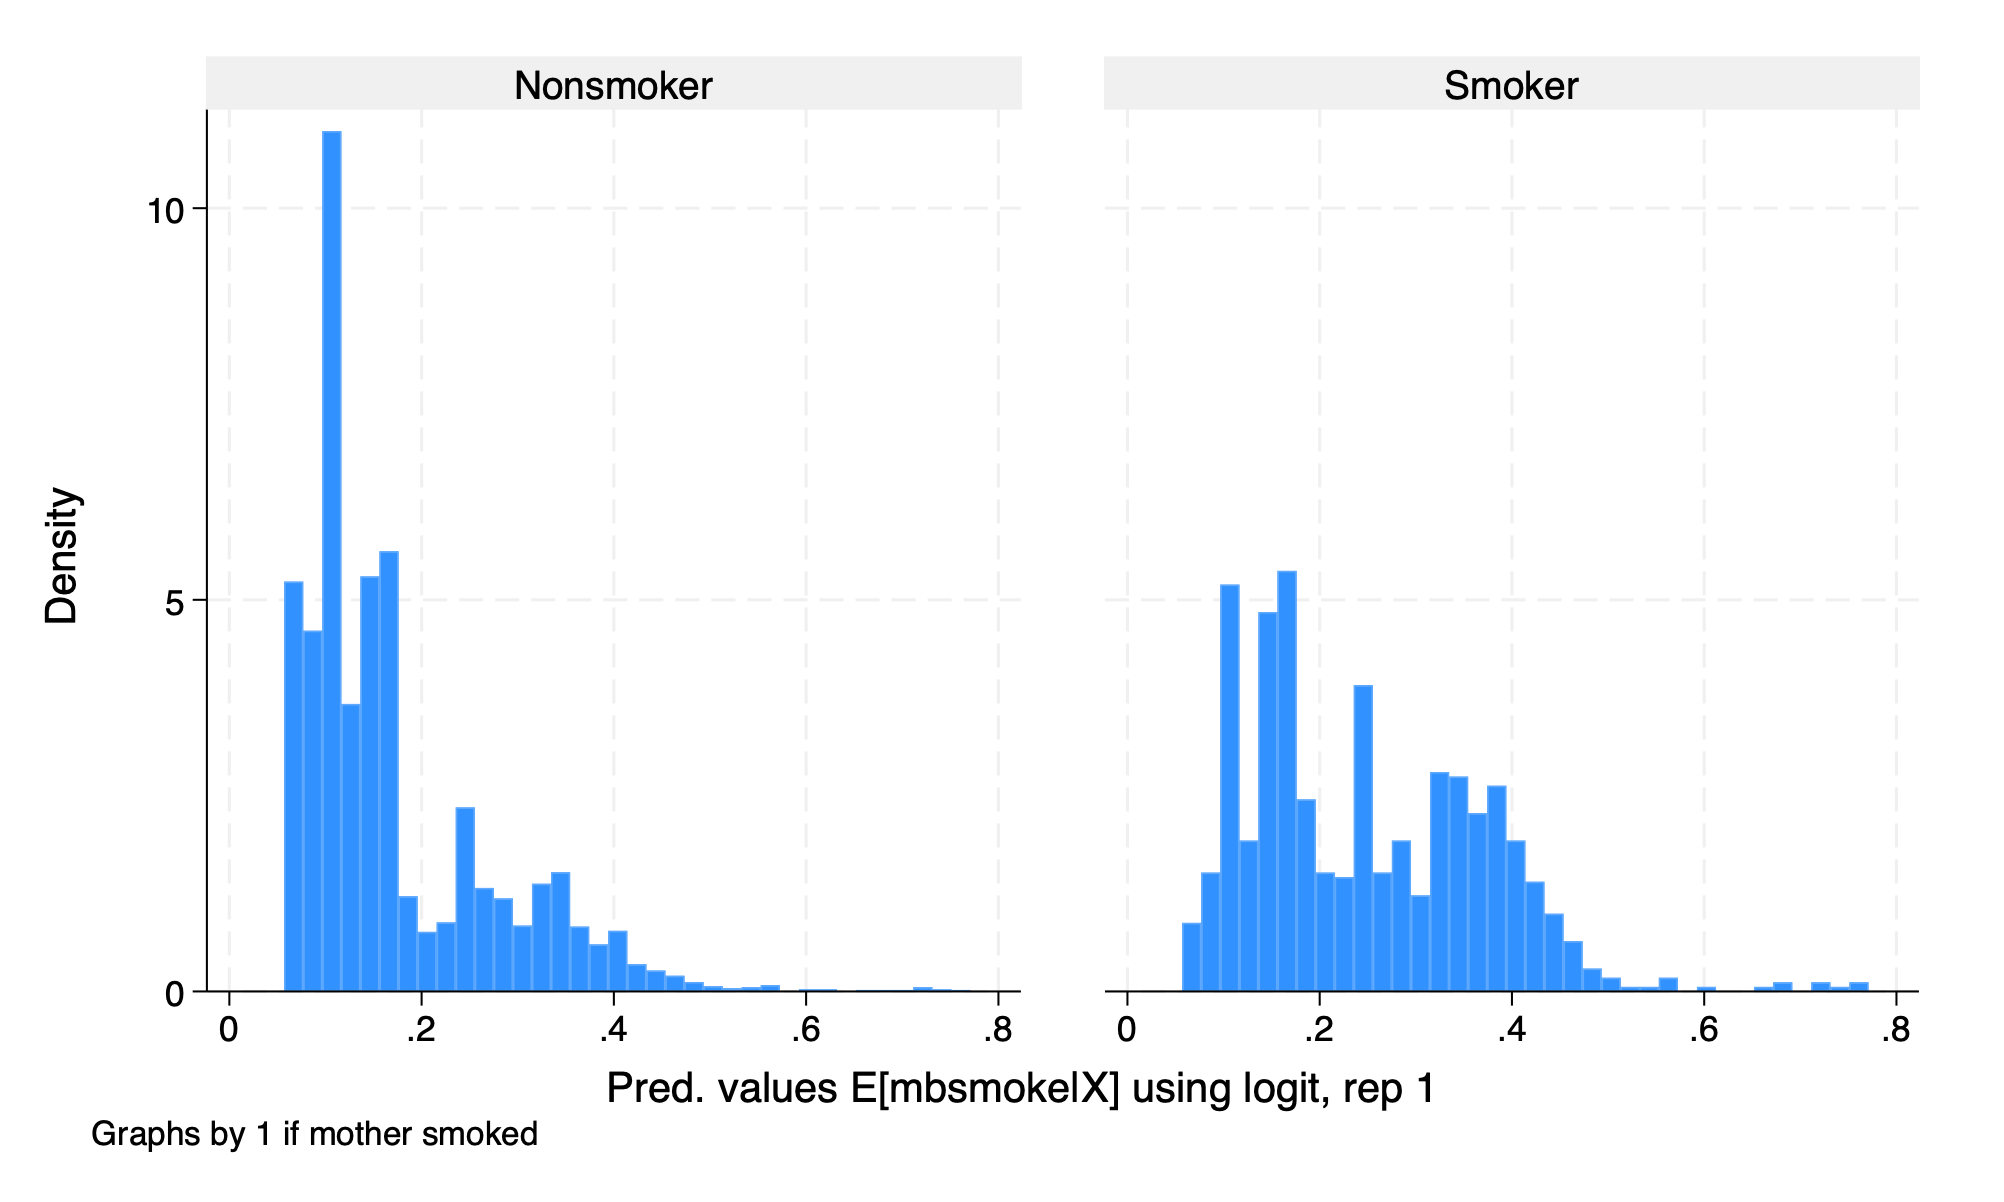
\includegraphics[keepaspectratio,alt={Estimated \textbackslash hat\{p\}-scores using logit}]{Smoke_logit_histogram.png}}
\caption{Estimated \(\hat{p}\)-scores using logit}
\end{figure}

\begin{figure}
\centering
\pandocbounded{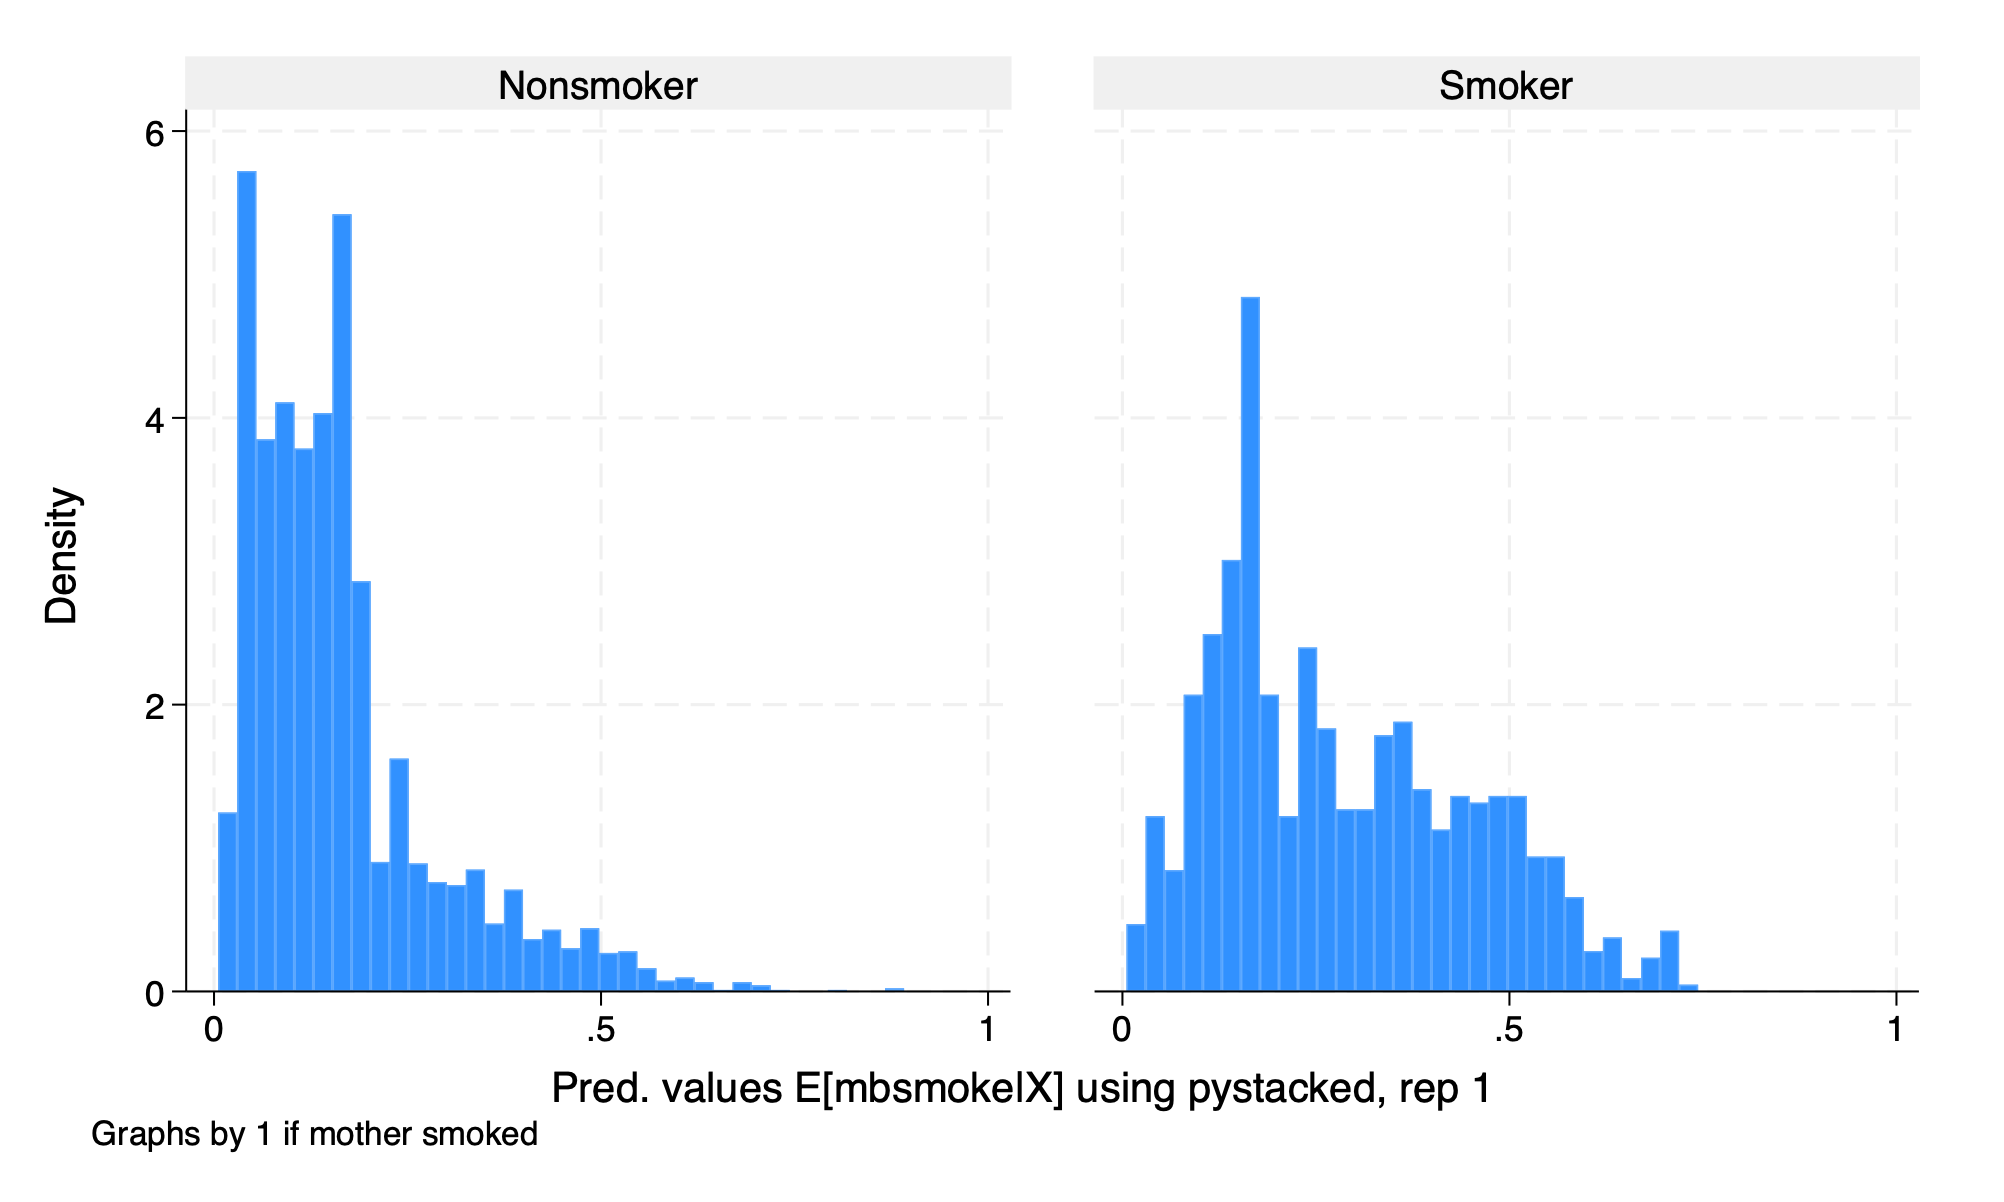
\includegraphics[keepaspectratio,alt={Estimated \textbackslash hat\{p\}-scores using Gradient Boost}]{Smoke_gradboost_histogram.png}}
\caption{Estimated \(\hat{p}\)-scores using Gradient Boost}
\end{figure}

\section{Estimation}\label{estimation-1}

After our crossfitting/crossvalidation to test the model, we can now estimate our parameters of interest, which are the \(ATE\) and the \(ATET\).

\begin{Shaded}
\begin{Highlighting}[]
\NormalTok{ddml estimate, ate allcombos}
\NormalTok{ddml estimate, atet allcombos}
\end{Highlighting}
\end{Shaded}

\begin{verbatim}
Model:                  interactive, crossfit folds k=5, resamples r=5
Mata global (mname):    m0
Dependent variable (Y): bweight
 bweight learners:      Y1_reg Y2_pystacked
D equations (1):        mbsmoke
 mbsmoke learners:      D1_logit D2_pystacked

DDML estimation results (ATE):
spec  r  Y(0) learner  Y(1) learner     D learner         b        SE 
   1  1        Y1_reg        Y1_reg      D1_logit  -232.439   (23.705)
   2  1        Y1_reg        Y1_reg  D2_pystacked  -207.548   (32.276)
   3  1        Y1_reg  Y2_pystacked      D1_logit  -232.489   (23.790)
   4  1        Y1_reg  Y2_pystacked  D2_pystacked  -209.111   (32.570)
   5  1  Y2_pystacked        Y1_reg      D1_logit  -232.413   (23.705)
*  6  1  Y2_pystacked        Y1_reg  D2_pystacked  -207.534   (32.276)
   7  1  Y2_pystacked  Y2_pystacked      D1_logit  -232.464   (23.791)
   8  1  Y2_pystacked  Y2_pystacked  D2_pystacked  -209.098   (32.571)
   1  2        Y1_reg        Y1_reg      D1_logit  -231.528   (23.962)
*  2  2        Y1_reg        Y1_reg  D2_pystacked  -212.120   (29.030)
   3  2        Y1_reg  Y2_pystacked      D1_logit  -232.670   (23.987)
   4  2        Y1_reg  Y2_pystacked  D2_pystacked  -212.830   (29.032)
   5  2  Y2_pystacked        Y1_reg      D1_logit  -231.548   (23.963)
   6  2  Y2_pystacked        Y1_reg  D2_pystacked  -212.143   (29.030)
   7  2  Y2_pystacked  Y2_pystacked      D1_logit  -232.690   (23.988)
   8  2  Y2_pystacked  Y2_pystacked  D2_pystacked  -212.852   (29.032)
   1  3        Y1_reg        Y1_reg      D1_logit  -232.185   (23.785)
   2  3        Y1_reg        Y1_reg  D2_pystacked  -227.979   (30.761)
   3  3        Y1_reg  Y2_pystacked      D1_logit  -234.067   (23.831)
   4  3        Y1_reg  Y2_pystacked  D2_pystacked  -230.055   (30.774)
   5  3  Y2_pystacked        Y1_reg      D1_logit  -232.160   (23.784)
*  6  3  Y2_pystacked        Y1_reg  D2_pystacked  -227.926   (30.761)
   7  3  Y2_pystacked  Y2_pystacked      D1_logit  -234.042   (23.831)
   8  3  Y2_pystacked  Y2_pystacked  D2_pystacked  -230.002   (30.773)
   1  4        Y1_reg        Y1_reg      D1_logit  -232.120   (23.741)
*  2  4        Y1_reg        Y1_reg  D2_pystacked  -216.024   (29.016)
   3  4        Y1_reg  Y2_pystacked      D1_logit  -234.314   (23.797)
   4  4        Y1_reg  Y2_pystacked  D2_pystacked  -218.391   (29.148)
   5  4  Y2_pystacked        Y1_reg      D1_logit  -232.131   (23.741)
   6  4  Y2_pystacked        Y1_reg  D2_pystacked  -216.039   (29.016)
   7  4  Y2_pystacked  Y2_pystacked      D1_logit  -234.325   (23.797)
   8  4  Y2_pystacked  Y2_pystacked  D2_pystacked  -218.406   (29.148)
   1  5        Y1_reg        Y1_reg      D1_logit  -232.445   (23.580)
*  2  5        Y1_reg        Y1_reg  D2_pystacked  -216.653   (29.485)
   3  5        Y1_reg  Y2_pystacked      D1_logit  -233.883   (23.689)
   4  5        Y1_reg  Y2_pystacked  D2_pystacked  -219.499   (29.507)
   5  5  Y2_pystacked        Y1_reg      D1_logit  -232.406   (23.580)
   6  5  Y2_pystacked        Y1_reg  D2_pystacked  -216.659   (29.486)
   7  5  Y2_pystacked  Y2_pystacked      D1_logit  -233.844   (23.689)
   8  5  Y2_pystacked  Y2_pystacked  D2_pystacked  -219.505   (29.507)
* = minimum MSE specification for that resample.

Mean/med Y(0) learner  Y(1) learner     D learner         b        SE 
   1 mn       Y1_reg0       Y1_reg1      D1_logit  -232.143   (23.756)
   1 md       Y1_reg0       Y1_reg1      D1_logit  -232.185   (23.741)
   2 mn       Y1_reg0       Y1_reg1  D2_pystacked  -216.065   (30.660)
   2 md       Y1_reg0       Y1_reg1  D2_pystacked  -216.024   (29.492)
   3 mn       Y1_reg0 Y2_pystacked1      D1_logit  -233.485   (23.830)
   3 md       Y1_reg0 Y2_pystacked1      D1_logit  -233.883   (23.831)
   4 mn       Y1_reg0 Y2_pystacked1  D2_pystacked  -217.977   (30.816)
   4 md       Y1_reg0 Y2_pystacked1  D2_pystacked  -218.391   (29.559)
   5 mn Y2_pystacked0       Y1_reg1      D1_logit  -232.132   (23.756)
   5 md Y2_pystacked0       Y1_reg1      D1_logit  -232.160   (23.741)
   6 mn Y2_pystacked0       Y1_reg1  D2_pystacked  -216.060   (30.657)
   6 md Y2_pystacked0       Y1_reg1  D2_pystacked  -216.039   (29.492)
   7 mn Y2_pystacked0 Y2_pystacked1      D1_logit  -233.473   (23.830)
   7 md Y2_pystacked0 Y2_pystacked1      D1_logit  -233.844   (23.831)
   8 mn Y2_pystacked0 Y2_pystacked1  D2_pystacked  -217.973   (30.813)
   8 md Y2_pystacked0 Y2_pystacked1  D2_pystacked  -218.406   (29.558)
 mse mn     [min-mse]     [min-mse]     [min-mse]  -216.052   (30.657)
 mse md     [min-mse]     [min-mse]     [min-mse]  -216.024   (29.492)

Median over 5 min-mse specifications (ATE)
E[y|X,D=0]   = md_0_mse                            Number of obs   =      4642
E[y|X,D=1]   = md_1_mse
E[D|X]       = md_mbsmoke_mse
------------------------------------------------------------------------------
             |               Robust
     bweight | Coefficient  std. err.      z    P>|z|     [95% conf. interval]
-------------+----------------------------------------------------------------
     mbsmoke |  -216.0236   29.49151    -7.32   0.000     -273.826   -158.2213
------------------------------------------------------------------------------
Warning: 5 resamples had propensity scores trimmed to lower limit .01.

Summary over 5 resamples:
       D eqn      mean       min       p25       p50       p75       max
     mbsmoke   -216.0516 -227.9261 -216.6534 -216.0237 -212.1205 -207.5342



Model:                  interactive, crossfit folds k=5, resamples r=5
Mata global (mname):    m0
Dependent variable (Y): bweight
 bweight learners:      Y1_reg Y2_pystacked
D equations (1):        mbsmoke
 mbsmoke learners:      D1_logit D2_pystacked

DDML estimation results (ATET):
spec  r  Y(0) learner  Y(1) learner     D learner         b        SE 
   1  1        Y1_reg        Y1_reg      D1_logit  -219.785   (23.719)
   2  1        Y1_reg        Y1_reg  D2_pystacked  -234.767   (24.667)
   3  1        Y1_reg  Y2_pystacked      D1_logit  -219.785   (23.719)
   4  1        Y1_reg  Y2_pystacked  D2_pystacked  -234.767   (24.667)
   5  1  Y2_pystacked        Y1_reg      D1_logit  -219.643   (23.711)
*  6  1  Y2_pystacked        Y1_reg  D2_pystacked  -234.692   (24.660)
   7  1  Y2_pystacked  Y2_pystacked      D1_logit  -219.643   (23.711)
   8  1  Y2_pystacked  Y2_pystacked  D2_pystacked  -234.692   (24.660)
   1  2        Y1_reg        Y1_reg      D1_logit  -219.674   (23.696)
*  2  2        Y1_reg        Y1_reg  D2_pystacked  -231.269   (25.229)
   3  2        Y1_reg  Y2_pystacked      D1_logit  -219.674   (23.696)
   4  2        Y1_reg  Y2_pystacked  D2_pystacked  -231.269   (25.229)
   5  2  Y2_pystacked        Y1_reg      D1_logit  -219.779   (23.698)
   6  2  Y2_pystacked        Y1_reg  D2_pystacked  -231.382   (25.228)
   7  2  Y2_pystacked  Y2_pystacked      D1_logit  -219.779   (23.698)
   8  2  Y2_pystacked  Y2_pystacked  D2_pystacked  -231.382   (25.228)
   1  3        Y1_reg        Y1_reg      D1_logit  -225.808   (23.697)
   2  3        Y1_reg        Y1_reg  D2_pystacked  -239.953   (24.672)
   3  3        Y1_reg  Y2_pystacked      D1_logit  -225.808   (23.697)
   4  3        Y1_reg  Y2_pystacked  D2_pystacked  -239.953   (24.672)
   5  3  Y2_pystacked        Y1_reg      D1_logit  -225.670   (23.681)
*  6  3  Y2_pystacked        Y1_reg  D2_pystacked  -239.672   (24.647)
   7  3  Y2_pystacked  Y2_pystacked      D1_logit  -225.670   (23.681)
   8  3  Y2_pystacked  Y2_pystacked  D2_pystacked  -239.672   (24.647)
   1  4        Y1_reg        Y1_reg      D1_logit  -222.562   (23.714)
*  2  4        Y1_reg        Y1_reg  D2_pystacked  -239.122   (24.476)
   3  4        Y1_reg  Y2_pystacked      D1_logit  -222.562   (23.714)
   4  4        Y1_reg  Y2_pystacked  D2_pystacked  -239.122   (24.476)
   5  4  Y2_pystacked        Y1_reg      D1_logit  -222.616   (23.707)
   6  4  Y2_pystacked        Y1_reg  D2_pystacked  -239.202   (24.468)
   7  4  Y2_pystacked  Y2_pystacked      D1_logit  -222.616   (23.707)
   8  4  Y2_pystacked  Y2_pystacked  D2_pystacked  -239.202   (24.468)
   1  5        Y1_reg        Y1_reg      D1_logit  -222.114   (23.395)
*  2  5        Y1_reg        Y1_reg  D2_pystacked  -234.163   (24.664)
   3  5        Y1_reg  Y2_pystacked      D1_logit  -222.114   (23.395)
   4  5        Y1_reg  Y2_pystacked  D2_pystacked  -234.163   (24.664)
   5  5  Y2_pystacked        Y1_reg      D1_logit  -221.898   (23.374)
   6  5  Y2_pystacked        Y1_reg  D2_pystacked  -234.193   (24.649)
   7  5  Y2_pystacked  Y2_pystacked      D1_logit  -221.898   (23.374)
   8  5  Y2_pystacked  Y2_pystacked  D2_pystacked  -234.193   (24.649)
* = minimum MSE specification for that resample.

Mean/med Y(0) learner  Y(1) learner     D learner         b        SE 
   1 mn       Y1_reg0       Y1_reg1      D1_logit  -221.989   (23.747)
   1 md       Y1_reg0       Y1_reg1      D1_logit  -222.114   (23.821)
   2 mn       Y1_reg0       Y1_reg1  D2_pystacked  -235.855   (24.944)
   2 md       Y1_reg0       Y1_reg1  D2_pystacked  -234.767   (24.860)
   3 mn       Y1_reg0 Y2_pystacked1      D1_logit  -221.989   (23.747)
   3 md       Y1_reg0 Y2_pystacked1      D1_logit  -222.114   (23.821)
   4 mn       Y1_reg0 Y2_pystacked1  D2_pystacked  -235.855   (24.944)
   4 md       Y1_reg0 Y2_pystacked1  D2_pystacked  -234.767   (24.860)
   5 mn Y2_pystacked0       Y1_reg1      D1_logit  -221.921   (23.734)
   5 md Y2_pystacked0       Y1_reg1      D1_logit  -221.898   (23.792)
   6 mn Y2_pystacked0       Y1_reg1  D2_pystacked  -235.828   (24.923)
   6 md Y2_pystacked0       Y1_reg1  D2_pystacked  -234.692   (24.881)
   7 mn Y2_pystacked0 Y2_pystacked1      D1_logit  -221.921   (23.734)
   7 md Y2_pystacked0 Y2_pystacked1      D1_logit  -221.898   (23.792)
   8 mn Y2_pystacked0 Y2_pystacked1  D2_pystacked  -235.828   (24.923)
   8 md Y2_pystacked0 Y2_pystacked1  D2_pystacked  -234.692   (24.881)
 mse mn     [min-mse]     [min-mse]     [min-mse]  -235.783   (24.929)
 mse md     [min-mse]     [min-mse]     [min-mse]  -234.692   (24.874)

Median over 5 min-mse specifications (ATET)
E[y|X,D=0]   = md_0_mse                            Number of obs   =      4642
E[y|X,D=1]   = md_1_mse
E[D|X]       = md_mbsmoke_mse
------------------------------------------------------------------------------
             |               Robust
     bweight | Coefficient  std. err.      z    P>|z|     [95% conf. interval]
-------------+----------------------------------------------------------------
     mbsmoke |  -234.6921   24.87355    -9.44   0.000    -283.4433   -185.9408
------------------------------------------------------------------------------
Warning: 5 resamples had propensity scores trimmed to lower limit .01.

Summary over 5 resamples:
       D eqn      mean       min       p25       p50       p75       max
     mbsmoke   -235.7835 -239.6716 -239.1219 -234.6921 -234.1633 -231.2686
\end{verbatim}

Our \(\widehat{ATE}\) is \(-216.024\) or smoking reduces birth weight of a baby by 213 grams, which is statistically significant at the \(5\%\) level.

Our \(\widehat{ATET}\) is \(-234.692\) or smoking reduces birth weight of a baby by 234 grams for the treatment group, which is statistically significant at the \(5\%\) level.

Please note that the median over the minimum-MSE specification per resampling iteration is shown in the output. Below the output is a table that shows summary statistics of the resampling iterations.

\chapter{Training Example Revisited}\label{training-example-revisited}

I want to revisit the training sample to show the importance of our second assumption of common support.

\section{Doubly Robust Estimator}\label{doubly-robust-estimator}

Let's reload the data and run our double robust estimator.

\begin{Shaded}
\begin{Highlighting}[]
\KeywordTok{quietly}\NormalTok{ \{}
\KeywordTok{use}\NormalTok{ https:}\CommentTok{//github.com/scunning1975/mixtape/raw/master/nsw\_mixtape.dta, clear}
\KeywordTok{drop} \KeywordTok{if}\NormalTok{ treat==0}

\NormalTok{* Now }\KeywordTok{merge} \KeywordTok{in}\NormalTok{ the CPS controls from footnote 2 }\KeywordTok{of}\NormalTok{ Table 2 (Dehejia and Wahba 2002)}
\KeywordTok{append} \KeywordTok{using}\NormalTok{ https:}\CommentTok{//github.com/scunning1975/mixtape/raw/master/cps\_mixtape.dta}
\KeywordTok{gen}\NormalTok{ agesq=age*age}
\KeywordTok{gen}\NormalTok{ agecube=age*age*age}
\KeywordTok{gen}\NormalTok{ edusq=educ*edu}
\KeywordTok{gen}\NormalTok{ u74 = 0 }\KeywordTok{if}\NormalTok{ re74!=.}
\KeywordTok{replace}\NormalTok{ u74 = 1 }\KeywordTok{if}\NormalTok{ re74==0}
\KeywordTok{gen}\NormalTok{ u75 = 0 }\KeywordTok{if}\NormalTok{ re75!=.}
\KeywordTok{replace}\NormalTok{ u75 = 1 }\KeywordTok{if}\NormalTok{ re75==0}
\KeywordTok{gen}\NormalTok{ interaction1 = educ*re74}
\KeywordTok{gen}\NormalTok{ re74sq=re74\^{}2}
\KeywordTok{gen}\NormalTok{ re75sq=re75\^{}2}
\KeywordTok{gen}\NormalTok{ interaction2 = u74*hisp}


\NormalTok{* Now estimate the propensity }\KeywordTok{score}
\KeywordTok{logit}\NormalTok{ treat age agesq agecube educ edusq marr nodegree }\BaseNTok{black}\NormalTok{ hisp re74 re75 u74 u75 interaction1 }
\KeywordTok{predict}\NormalTok{ pscore}

\NormalTok{* Checking }\KeywordTok{mean}\NormalTok{ propensity scores }\KeywordTok{for}\NormalTok{ treatment and control groups}
\KeywordTok{sum}\NormalTok{ pscore }\KeywordTok{if}\NormalTok{ treat==1, }\KeywordTok{detail}
\KeywordTok{sum}\NormalTok{ pscore }\KeywordTok{if}\NormalTok{ treat==0, }\KeywordTok{detail}

\NormalTok{* Now look }\FunctionTok{at}\NormalTok{ the propensity }\KeywordTok{score}\NormalTok{ distribution }\KeywordTok{for}\NormalTok{ treatment and control groups}
\KeywordTok{histogram}\NormalTok{ pscore, }\KeywordTok{by}\NormalTok{(treat) binrescale}

\NormalTok{* Trimming the propensity }\KeywordTok{score}
\KeywordTok{drop} \KeywordTok{if}\NormalTok{ pscore \textless{}= 0.1 }
\KeywordTok{drop} \KeywordTok{if}\NormalTok{ pscore \textgreater{}= 0.9}

\NormalTok{\}}
\NormalTok{*ATT}
\NormalTok{*We have to rescale }\KeywordTok{for}\NormalTok{ the concavity }\KeywordTok{of}\NormalTok{ the }\KeywordTok{logit}\NormalTok{.}
\KeywordTok{gen}\NormalTok{ re78\_scaled = re78/1000}

\NormalTok{teffects ipwra (re78\_scaled age agesq agecube educ edusq marr nodegree }\BaseNTok{black}\NormalTok{ hisp re74 re75 u74 u75 interaction1) (treat age agesq agecube educ edusq marr nodegree }\BaseNTok{black}\NormalTok{ hisp u74 u75 interaction1, }\KeywordTok{logit}\NormalTok{), atet}
\KeywordTok{capture} \KeywordTok{drop}\NormalTok{ overlap}

\NormalTok{*ATE}
\NormalTok{teffects ipwra (re78\_scaled age agesq agecube educ edusq marr nodegree }\BaseNTok{black}\NormalTok{ hisp re74 re75 u74 u75 interaction1) (treat age agesq agecube educ edusq marr nodegree }\BaseNTok{black}\NormalTok{ hisp u74 u75 interaction1, }\KeywordTok{logit}\NormalTok{), ate}
\end{Highlighting}
\end{Shaded}

\begin{verbatim}
Iteration 0:  EE criterion = 3.017e-21  
Iteration 1:  EE criterion = 7.330e-29  

Treatment-effects estimation                    Number of obs     =        361
Estimator      : IPW regression adjustment
Outcome model  : linear
Treatment model: logit
------------------------------------------------------------------------------
             |               Robust
 re78_scaled | Coefficient  std. err.      z    P>|z|     [95% conf. interval]
-------------+----------------------------------------------------------------
ATET         |
       treat |
   (1 vs 0)  |   2.565509   .8702431     2.95   0.003     .8598639    4.271154
-------------+----------------------------------------------------------------
POmean       |
       treat |
          0  |   3.873287   .4696333     8.25   0.000     2.952823    4.793752
------------------------------------------------------------------------------



Iteration 0:  EE criterion = 2.997e-21  
Iteration 1:  EE criterion = 1.369e-28  

Treatment-effects estimation                    Number of obs     =        361
Estimator      : IPW regression adjustment
Outcome model  : linear
Treatment model: logit
------------------------------------------------------------------------------
             |               Robust
 re78_scaled | Coefficient  std. err.      z    P>|z|     [95% conf. interval]
-------------+----------------------------------------------------------------
ATE          |
       treat |
   (1 vs 0)  |   1.608922   .6988993     2.30   0.021     .2391044    2.978739
-------------+----------------------------------------------------------------
POmean       |
       treat |
          0  |   4.297229   .3749753    11.46   0.000     3.562291    5.032167
------------------------------------------------------------------------------
\end{verbatim}

Our estimate \(\widehat{ATE}\) is \(\$1,609\), and the estimate \(\widehat{ATET}\) is estimated \(\$2,566\). Recall that we need to trim our \(p\)-scores to satisfy the common support/overlap assumption.

\section{DDML Estimator}\label{ddml-estimator}

Let's rerun this, but we will use lasso and gradient boost for our training models along side OLS and logit.

\begin{Shaded}
\begin{Highlighting}[]
\KeywordTok{quietly}\NormalTok{ \{}
\KeywordTok{macro} \KeywordTok{drop} \DataTypeTok{\_all}

\KeywordTok{use}\NormalTok{ https:}\CommentTok{//github.com/scunning1975/mixtape/raw/master/nsw\_mixtape.dta, clear}
\KeywordTok{drop} \KeywordTok{if}\NormalTok{ treat==0}

\NormalTok{* Now }\KeywordTok{merge} \KeywordTok{in}\NormalTok{ the CPS controls from footnote 2 }\KeywordTok{of}\NormalTok{ Table 2 (Dehejia and Wahba 2002)}
\KeywordTok{append} \KeywordTok{using}\NormalTok{ https:}\CommentTok{//github.com/scunning1975/mixtape/raw/master/cps\_mixtape.dta}
\KeywordTok{gen}\NormalTok{ agesq=age*age}
\KeywordTok{gen}\NormalTok{ agecube=age*age*age}
\KeywordTok{gen}\NormalTok{ edusq=educ*edu}
\KeywordTok{gen}\NormalTok{ u74 = 0 }\KeywordTok{if}\NormalTok{ re74!=.}
\KeywordTok{replace}\NormalTok{ u74 = 1 }\KeywordTok{if}\NormalTok{ re74==0}
\KeywordTok{gen}\NormalTok{ u75 = 0 }\KeywordTok{if}\NormalTok{ re75!=.}
\KeywordTok{replace}\NormalTok{ u75 = 1 }\KeywordTok{if}\NormalTok{ re75==0}
\KeywordTok{gen}\NormalTok{ interaction1 = educ*re74}
\KeywordTok{gen}\NormalTok{ re74sq=re74\^{}2}
\KeywordTok{gen}\NormalTok{ re75sq=re75\^{}2}
\KeywordTok{gen}\NormalTok{ interaction2 = u74*hisp}

\KeywordTok{gen}\NormalTok{ re78\_scaled = re78/1000}

\KeywordTok{global}\NormalTok{ Y re78\_scaled}
\KeywordTok{global}\NormalTok{ D treat}
\KeywordTok{global}\NormalTok{ X age agesq agecube educ edusq marr nodegree }\BaseNTok{black}\NormalTok{ hisp re74 re75 u74 u75 interaction1}
\KeywordTok{set} \DecValTok{seed}\NormalTok{ 123456}
\KeywordTok{display} \StringTok{"$X"}
\NormalTok{\}}
\NormalTok{ddml init interactive, kfolds(5)}

\NormalTok{ddml E[Y|X,D]: }\KeywordTok{reg} \OtherTok{$Y} \OtherTok{$X}
\NormalTok{ddml E[Y|X,D]: pystacked }\OtherTok{$Y} \OtherTok{$X}\NormalTok{, }\DecValTok{type}\NormalTok{(}\KeywordTok{reg}\NormalTok{) method(lassocv)}
\NormalTok{ddml E[D|X]: }\KeywordTok{logit} \OtherTok{$D} \OtherTok{$X}
\NormalTok{ddml E[D|X]: pystacked }\OtherTok{$D} \OtherTok{$X}\NormalTok{, }\DecValTok{type}\NormalTok{(}\KeywordTok{class}\NormalTok{) method(gradboost)}

\NormalTok{ddml crossfit}

\KeywordTok{bysort}\NormalTok{ treat: }\KeywordTok{summarize}\NormalTok{ D1\_logit, }\KeywordTok{detail}
\KeywordTok{bysort}\NormalTok{ treat: }\KeywordTok{summarize}\NormalTok{ D2\_pystacked, }\KeywordTok{detail}
\end{Highlighting}
\end{Shaded}

\begin{verbatim}
Learner Y1_reg added successfully.

Learner Y2_pystacked added successfully.

Learner D1_logit added successfully.

Learner D2_pystacked added successfully.

Cross-fitting E[y|X,D] equation: re78_scaled
Cross-fitting fold 1 2 3 4 5 ...completed cross-fitting
Cross-fitting E[D|X] equation: treat
Cross-fitting fold 1 2 3 4 5 ...completed cross-fitting


----------------------------------------------------------------------------------
-> treat = 0

         Pred. values E[treat|X] using logit, rep 1
-------------------------------------------------------------
      Percentiles      Smallest
 1%     4.10e-07       8.30e-11
 5%     1.43e-06       2.42e-10
10%     2.92e-06       8.97e-10       Obs              15,992
25%     .0000162       2.07e-09       Sum of wgt.      15,992

50%     .0001114                      Mean           .0067867
                        Largest       Std. dev.      .0432812
75%     .0009588       .8752542
90%     .0065014       .9023648       Variance       .0018733
95%     .0163545        .919232       Skewness       12.33715
99%     .1673345       .9519283       Kurtosis        189.019

----------------------------------------------------------------------------------
-> treat = 1

         Pred. values E[treat|X] using logit, rep 1
-------------------------------------------------------------
      Percentiles      Smallest
 1%     .0007289       .0005851
 5%     .0054053       .0007289
10%      .018033       .0009342       Obs                 185
25%     .0934181       .0015951       Sum of wgt.         185

50%     .3965528                      Mean           .4155009
                        Largest       Std. dev.      .3162217
75%     .6564633       .9384993
90%     .8898593       .9412911       Variance       .0999962
95%     .9193571       .9505891       Skewness       .2252374
99%     .9505891       .9577641       Kurtosis       1.698453



----------------------------------------------------------------------------------
-> treat = 0

       Pred. values E[treat|X] using pystacked, rep 1
-------------------------------------------------------------
      Percentiles      Smallest
 1%     .0000436       .0000222
 5%     .0000746       .0000225
10%     .0001128       .0000237       Obs              15,992
25%      .000179       .0000258       Sum of wgt.      15,992

50%     .0003444                      Mean           .0065602
                        Largest       Std. dev.      .0489033
75%     .0010962       .9835668
90%     .0040418       .9846331       Variance       .0023915
95%     .0113463       .9934209       Skewness       13.19906
99%     .1583603       .9963998       Kurtosis        205.557

----------------------------------------------------------------------------------
-> treat = 1

       Pred. values E[treat|X] using pystacked, rep 1
-------------------------------------------------------------
      Percentiles      Smallest
 1%      .000392       .0002826
 5%     .0036306        .000392
10%     .0083862       .0006855       Obs                 185
25%     .0616826       .0011451       Sum of wgt.         185

50%     .3462951                      Mean           .4155527
                        Largest       Std. dev.      .3432286
75%     .6983553        .982987
90%      .943571        .983358       Variance       .1178059
95%     .9622306       .9874787       Skewness       .3037242
99%     .9874787       .9874787       Kurtosis       1.653423
\end{verbatim}

We can see that our \(\hat{p}\)-scores are quiet different between treatment and comparison groups. We saw this last week with our matching methods for this training example.

Let's graph our histograms by \(\hat{p}\)-scores

\begin{Shaded}
\begin{Highlighting}[]
\KeywordTok{histogram}\NormalTok{ D1\_logit\_1, }\KeywordTok{by}\NormalTok{(treat) }\BaseNTok{title}\NormalTok{(}\StringTok{"Using Logit"}\NormalTok{)}
\KeywordTok{graph} \KeywordTok{export} \StringTok{"/Users/Sam/Desktop/Econ 672/Bookdown/Week5/Train\_logit\_histogram.png"}\NormalTok{, }\KeywordTok{replace}
\end{Highlighting}
\end{Shaded}

\begin{figure}
\centering
\pandocbounded{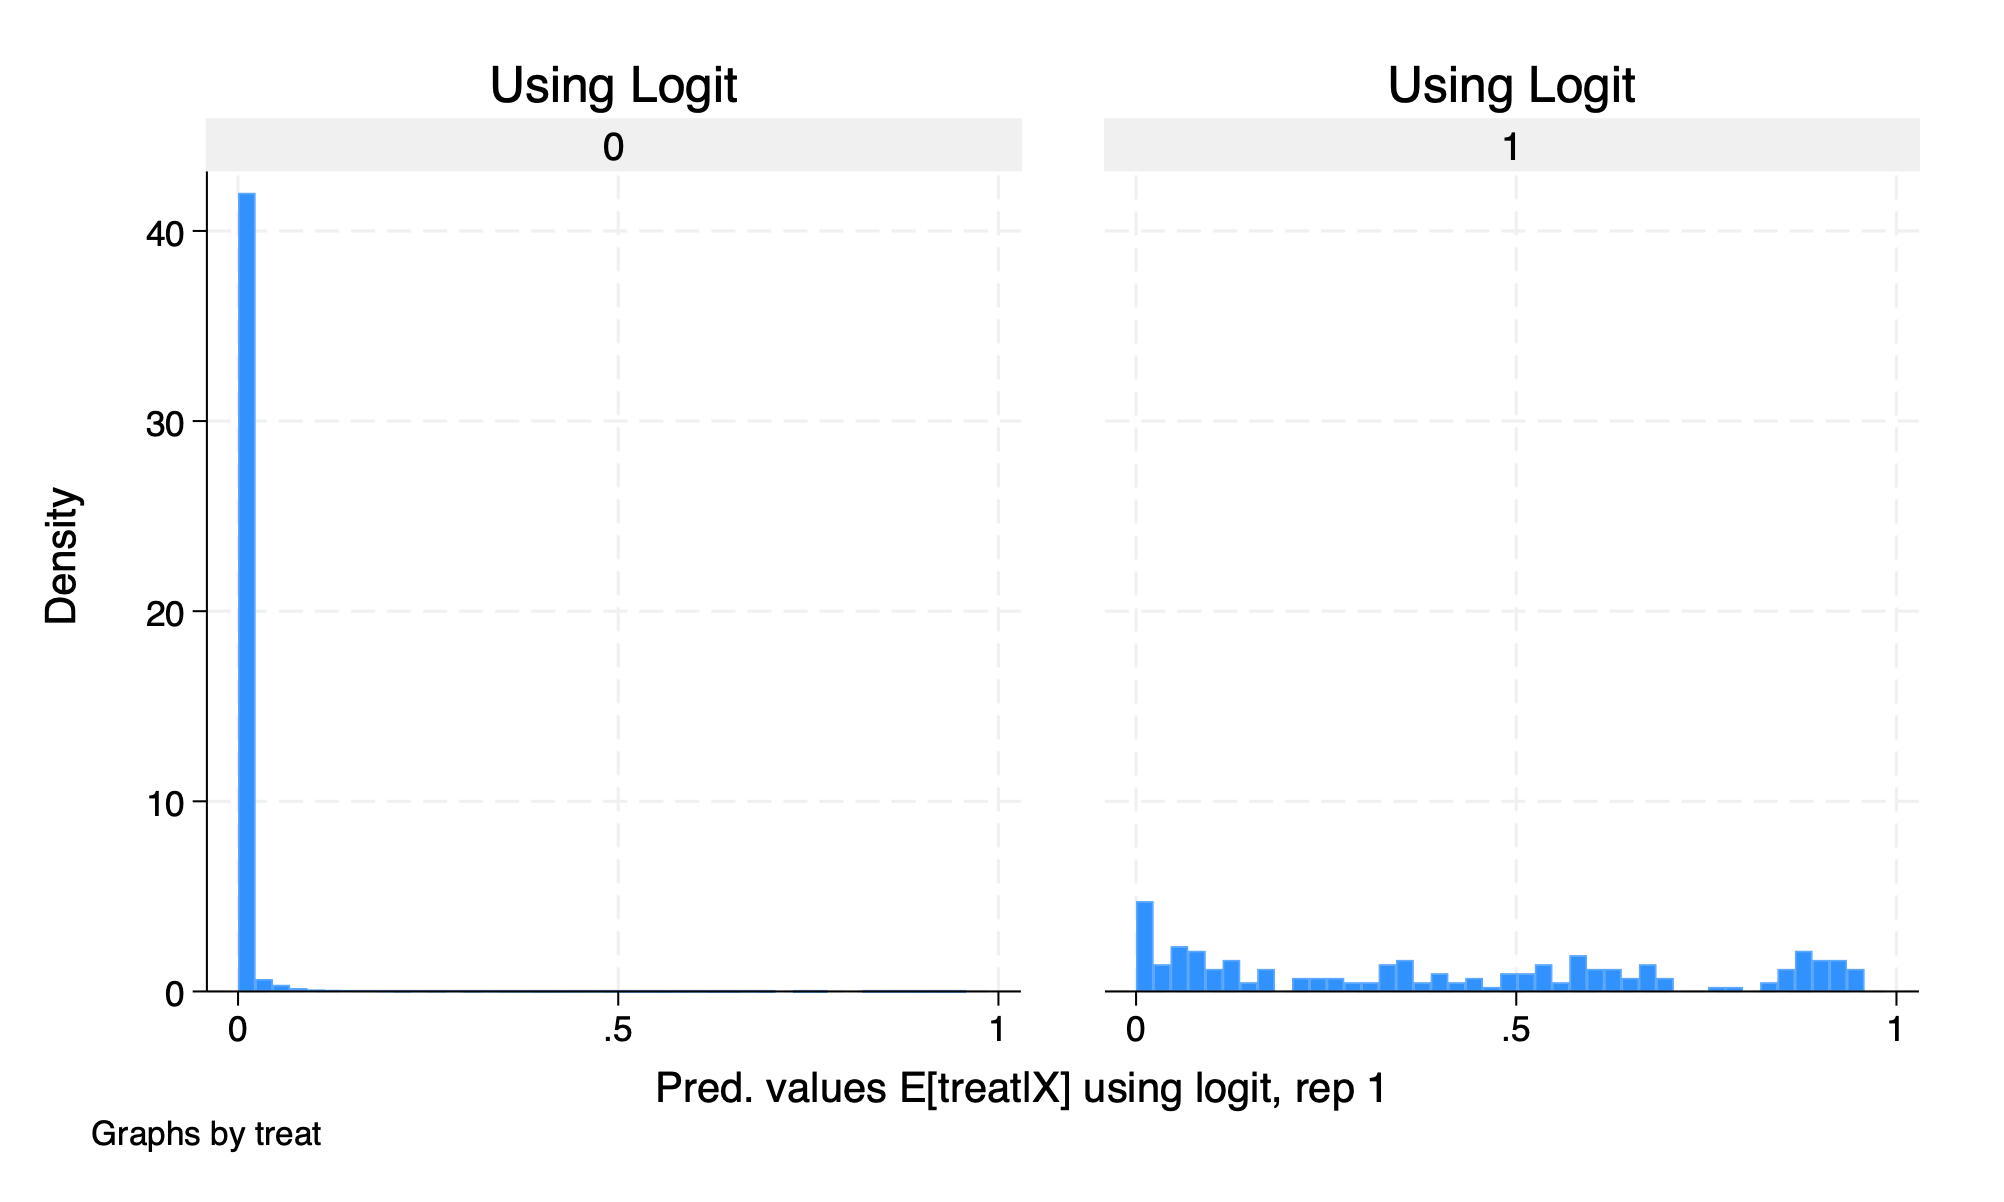
\includegraphics[keepaspectratio,alt={Histogram of \textbackslash hat\{p\}-scores using Logit}]{Train_logit_histogram.png}}
\caption{Histogram of \(\hat{p}\)-scores using Logit}
\end{figure}

\begin{Shaded}
\begin{Highlighting}[]
\KeywordTok{histogram}\NormalTok{ D2\_pystacked\_1, }\KeywordTok{by}\NormalTok{(treat) }\BaseNTok{title}\NormalTok{ (}\StringTok{"Using Gradient Boost"}\NormalTok{)}
\KeywordTok{graph} \KeywordTok{export} \StringTok{"/Users/Sam/Desktop/Econ 672/Bookdown/Week5/Train\_gradboost\_histogram.png"}\NormalTok{, }\KeywordTok{replace}
\end{Highlighting}
\end{Shaded}

\begin{figure}
\centering
\pandocbounded{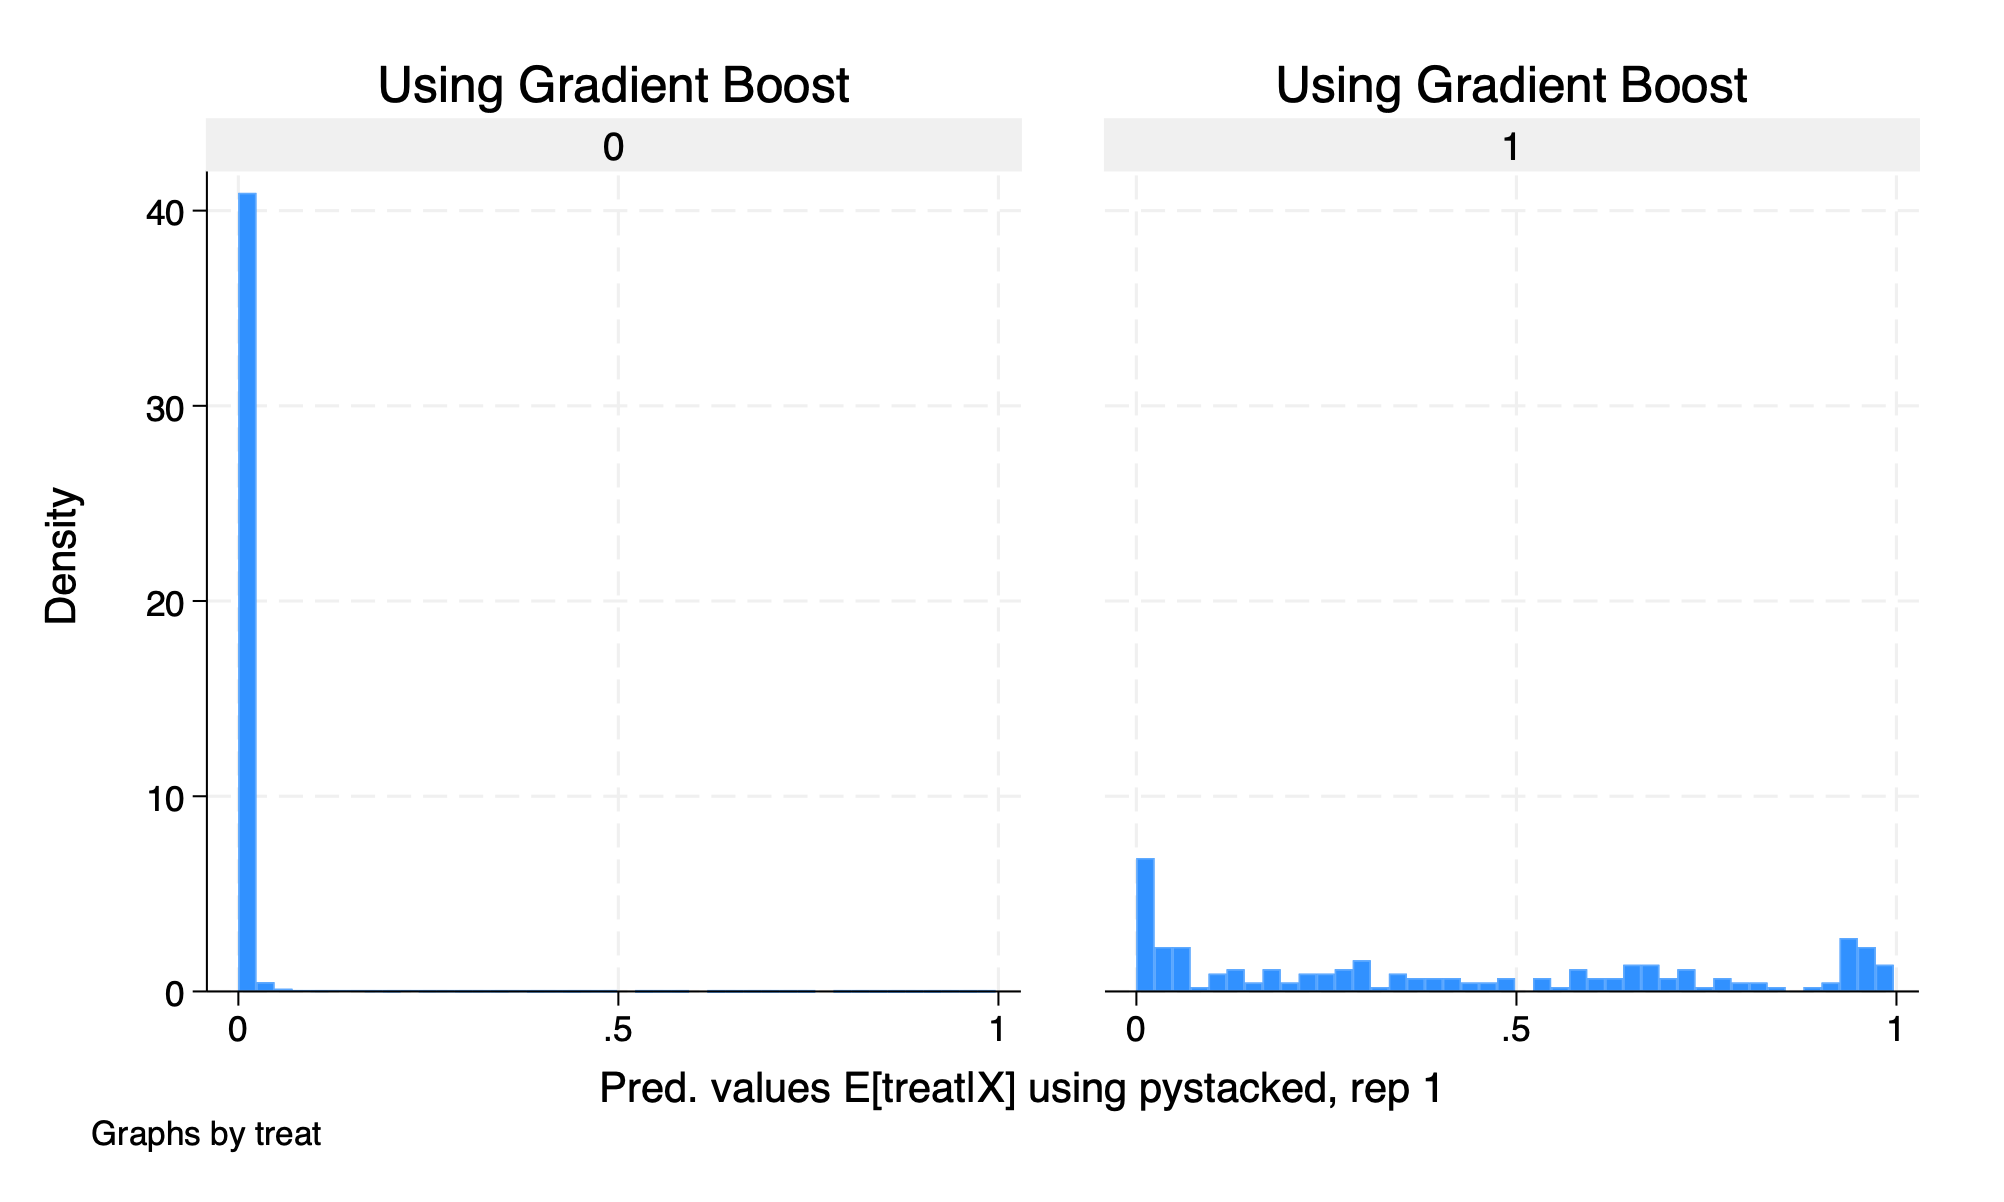
\includegraphics[keepaspectratio,alt={Histogram of \textbackslash hat\{p\}-scores using Gradient Boost}]{Train_gradboost_histogram.png}}
\caption{Histogram of \(\hat{p}\)-scores using Gradient Boost}
\end{figure}

We see that our common support assumption is violated. Let's run our estimate using DDML without trimming.

\begin{Shaded}
\begin{Highlighting}[]
\NormalTok{ddml estimate, allcombos }\KeywordTok{robust}
\end{Highlighting}
\end{Shaded}

\begin{verbatim}
Model:                  interactive, crossfit folds k=5, resamples r=1
Mata global (mname):    m0
Dependent variable (Y): re78_scaled
 re78_scaled learners:  Y1_reg Y2_pystacked
D equations (1):        treat
 treat learners:        D1_logit D2_pystacked

DDML estimation results (ATE):
spec  r  Y(0) learner  Y(1) learner     D learner         b        SE 
   1  1        Y1_reg        Y1_reg      D1_logit    -4.291    (0.283)
   2  1        Y1_reg        Y1_reg  D2_pystacked    -4.654    (0.255)
*  3  1        Y1_reg  Y2_pystacked      D1_logit    -6.440    (0.262)
   4  1        Y1_reg  Y2_pystacked  D2_pystacked    -6.758    (0.232)
   5  1  Y2_pystacked        Y1_reg      D1_logit    -4.290    (0.283)
   6  1  Y2_pystacked        Y1_reg  D2_pystacked    -4.646    (0.254)
   7  1  Y2_pystacked  Y2_pystacked      D1_logit    -6.439    (0.262)
   8  1  Y2_pystacked  Y2_pystacked  D2_pystacked    -6.750    (0.231)
* = minimum MSE specification for that resample.

Min MSE DDML model, specification 3 (ATE)
E[y|X,D=0]   = Y1_reg0_1                           Number of obs   =     16177
E[y|X,D=1]   = Y2_pystacked1
E[D|X]       = D1_logit_1
------------------------------------------------------------------------------
             |               Robust
 re78_scaled | Coefficient  std. err.      z    P>|z|     [95% conf. interval]
-------------+----------------------------------------------------------------
       treat |  -6.440495    .261945   -24.59   0.000    -6.953898   -5.927092
------------------------------------------------------------------------------
Warning: 14838 propensity scores trimmed to lower limit .01.
\end{verbatim}

Our estimated \(\widehat{ATE}\) is \(-\$6,440\), which is a far cry from our RCT estimate.

\section{Trimming}\label{trimming}

Let's do some trimming. Our model shows that the logit has a lower MSE than the gradiant boost, so we will use that first and then show our estimate with the

\begin{Shaded}
\begin{Highlighting}[]
\KeywordTok{histogram}\NormalTok{ D1\_logit\_1 }\KeywordTok{if}\NormalTok{ D1\_logit\_1 \textgreater{}.1 \& D1\_logit\_1 \textless{}.9, }\KeywordTok{by}\NormalTok{(treat) }\BaseNTok{title}\NormalTok{(Logit with Trimming)}
\KeywordTok{graph} \KeywordTok{export} \StringTok{"/Users/Sam/Desktop/Econ 672/Bookdown/Week5/Train\_logit\_histogram\_trimmed.png"}\NormalTok{, }\KeywordTok{replace}
\end{Highlighting}
\end{Shaded}

\begin{figure}
\centering
\pandocbounded{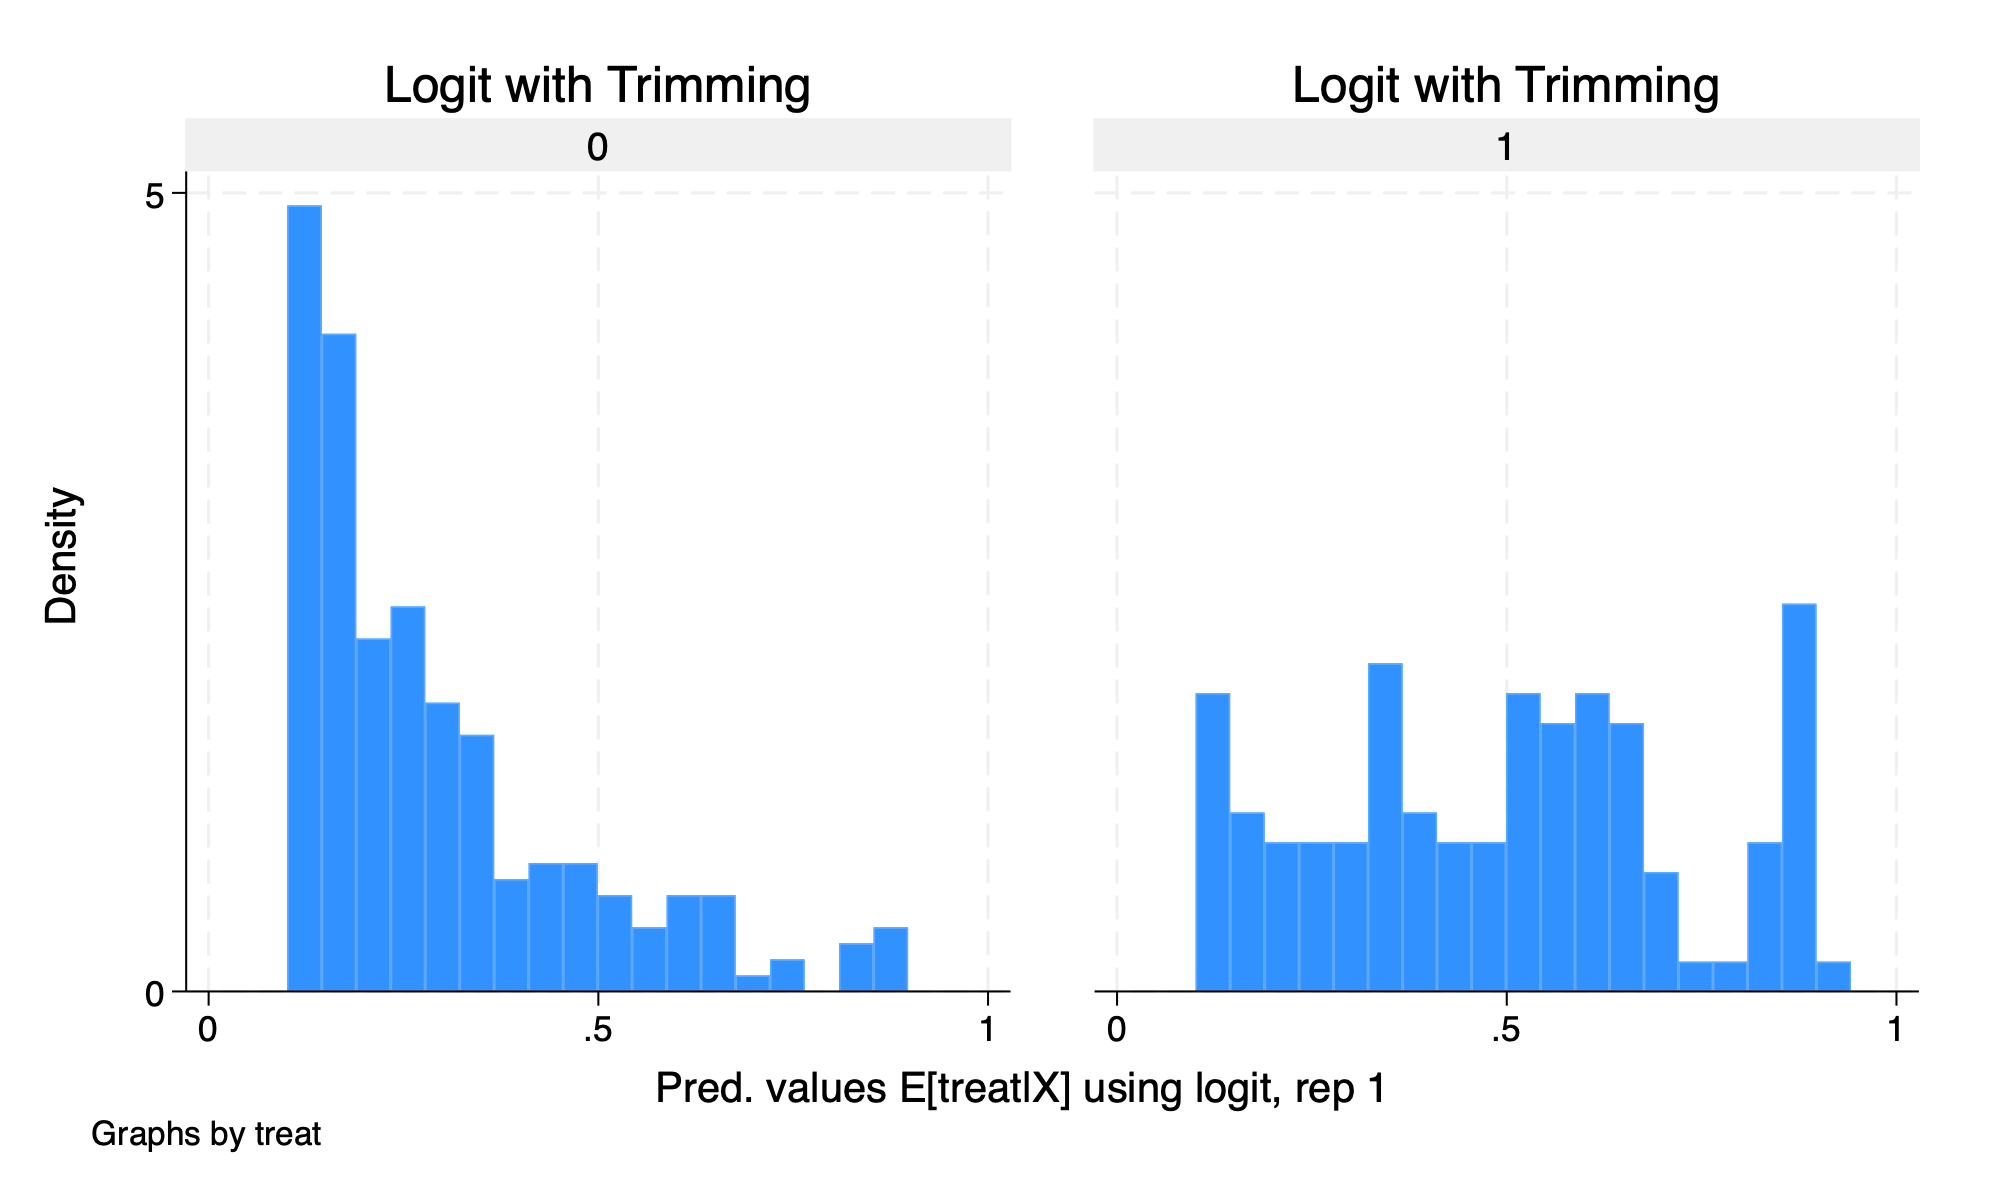
\includegraphics[keepaspectratio,alt={Histogram of \textbackslash hat\{p\}-scores with logit trimmed}]{Train_logit_histogram_trimmed.png}}
\caption{Histogram of \(\hat{p}\)-scores with logit trimmed}
\end{figure}

\begin{Shaded}
\begin{Highlighting}[]
\KeywordTok{histogram}\NormalTok{ D2\_pystacked\_1 }\KeywordTok{if}\NormalTok{ D2\_pystacked\_1 \textgreater{}.1 \& D2\_pystacked\_1 \textless{}.9, }\KeywordTok{by}\NormalTok{(treat) }\BaseNTok{title}\NormalTok{(Gradient Boost with Trimming)}
\KeywordTok{graph} \KeywordTok{export} \StringTok{"/Users/Sam/Desktop/Econ 672/Bookdown/Week5/Train\_gradboost\_histogram\_trimmed.png"}\NormalTok{, }\KeywordTok{replace}
\end{Highlighting}
\end{Shaded}

\begin{figure}
\centering
\pandocbounded{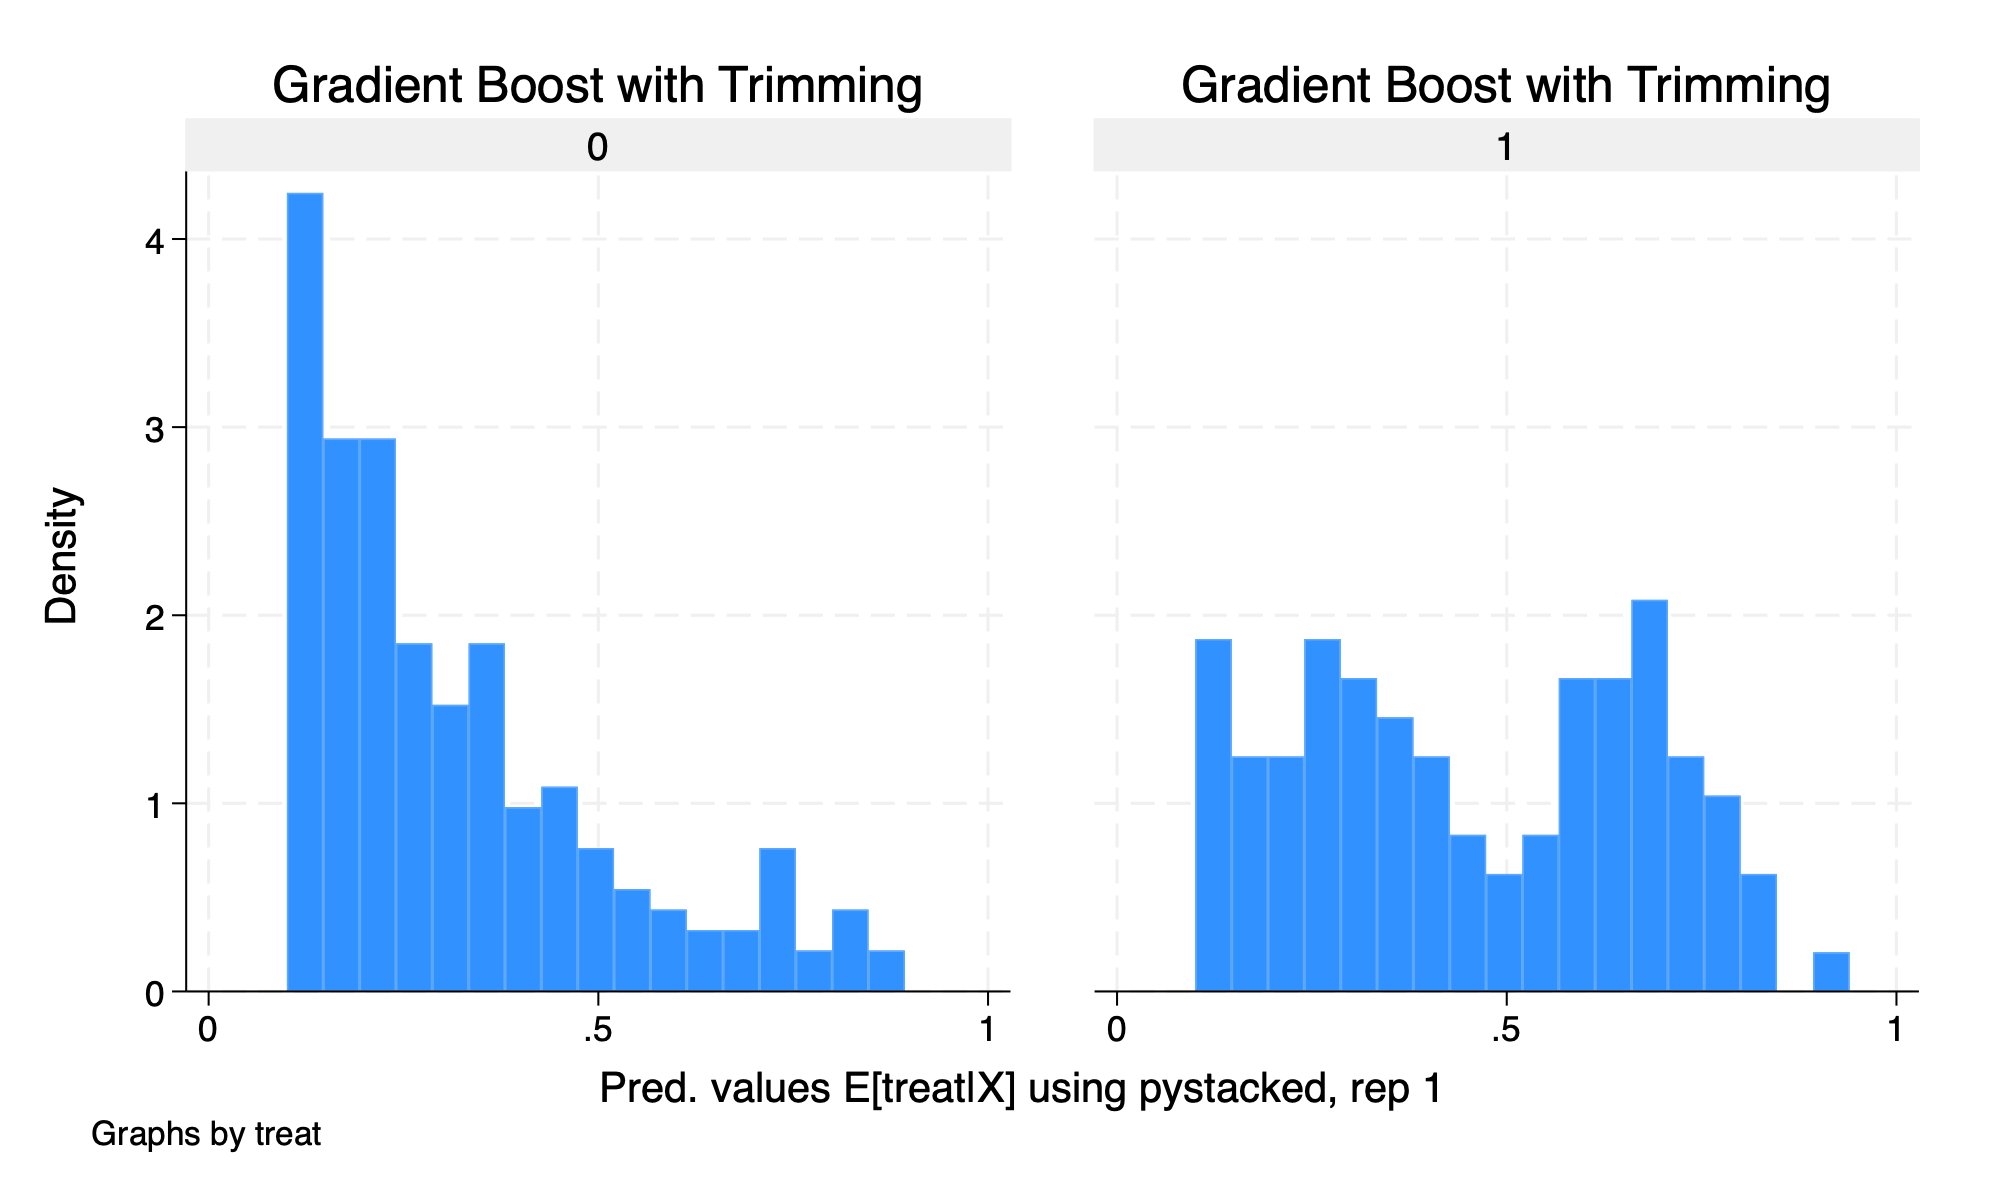
\includegraphics[keepaspectratio,alt={Histogram of \textbackslash hat\{p\}-scores with gradient boost trimmed}]{Train_gradboost_histogram_trimmed.png}}
\caption{Histogram of \(\hat{p}\)-scores with gradient boost trimmed}
\end{figure}

Let's rerun our estimate but with trimmed data.

\begin{Shaded}
\begin{Highlighting}[]
\NormalTok{ddml estimate }\KeywordTok{if}\NormalTok{ D1\_logit\_1 \textgreater{} .1 \& D1\_logit\_1 \textless{} .9, allcombos }\KeywordTok{robust}
\end{Highlighting}
\end{Shaded}

\begin{verbatim}
Model:                  interactive, crossfit folds k=5, resamples r=1
Mata global (mname):    m0
Dependent variable (Y): re78_scaled
 re78_scaled learners:  Y1_reg Y2_pystacked
D equations (1):        treat
 treat learners:        D1_logit D2_pystacked

DDML estimation results (ATE):
spec  r  Y(0) learner  Y(1) learner     D learner         b        SE 
   1  1        Y1_reg        Y1_reg      D1_logit     1.338    (0.965)
   2  1        Y1_reg        Y1_reg  D2_pystacked    -1.854    (3.334)
*  3  1        Y1_reg  Y2_pystacked      D1_logit     1.423    (0.860)
   4  1        Y1_reg  Y2_pystacked  D2_pystacked    -1.312    (2.536)
   5  1  Y2_pystacked        Y1_reg      D1_logit     1.359    (0.963)
   6  1  Y2_pystacked        Y1_reg  D2_pystacked    -1.776    (3.338)
   7  1  Y2_pystacked  Y2_pystacked      D1_logit     1.444    (0.858)
   8  1  Y2_pystacked  Y2_pystacked  D2_pystacked    -1.234    (2.542)
* = minimum MSE specification for that resample.

Min MSE DDML model, specification 3 (ATE)
E[y|X,D=0]   = Y1_reg0_1                           Number of obs   =       346
E[y|X,D=1]   = Y2_pystacked1
E[D|X]       = D1_logit_1
------------------------------------------------------------------------------
             |               Robust
 re78_scaled | Coefficient  std. err.      z    P>|z|     [95% conf. interval]
-------------+----------------------------------------------------------------
       treat |   1.423175   .8597525     1.66   0.098    -.2619087    3.108259
------------------------------------------------------------------------------
\end{verbatim}

Our estimated \(\hat{ATE}\) is \(\$1,423\), which is below our DR estimate and the RCT estimate and it is not statistically significant at the \(5\%\) level.

Ahrens, A. (2026). \emph{Setting Up Stata's Python Integration}. Stata ML Page. \url{https://statalasso.github.io}

Ahrens, Hansen, Scha↵er, and Wiemann (2023). \emph{DDML: Double/debiased machine learning in Stata}. Retrieved from: \url{https://docs.iza.org/dp15963.pdf}

Cunningham, S. (2021). \emph{Causal Inference: The Mixtape}. Yale University Press.

Huber, M. (2023). \emph{Causal Analysis: Impact Evaluation and Causal Machine Learning with Applications in R}. The MIT Press.

Huntington-Klein, N. (2022). \emph{The Effect: An Introduction to Research Design and Causality}. CRC Press.

\bibliography{book.bib,packages.bib}

\end{document}
